\chapter{Gather the Fruit}

The objective of this game is for the player to catch the falling fruits to prevent them from falling to the ground. For each fallen fruit, he loses a life. For each fruit caught, he earns one point. It's game over when you lose your three lives. The goal is to collect the maximum number of points.

\begin{figure}[H]
   \centering
   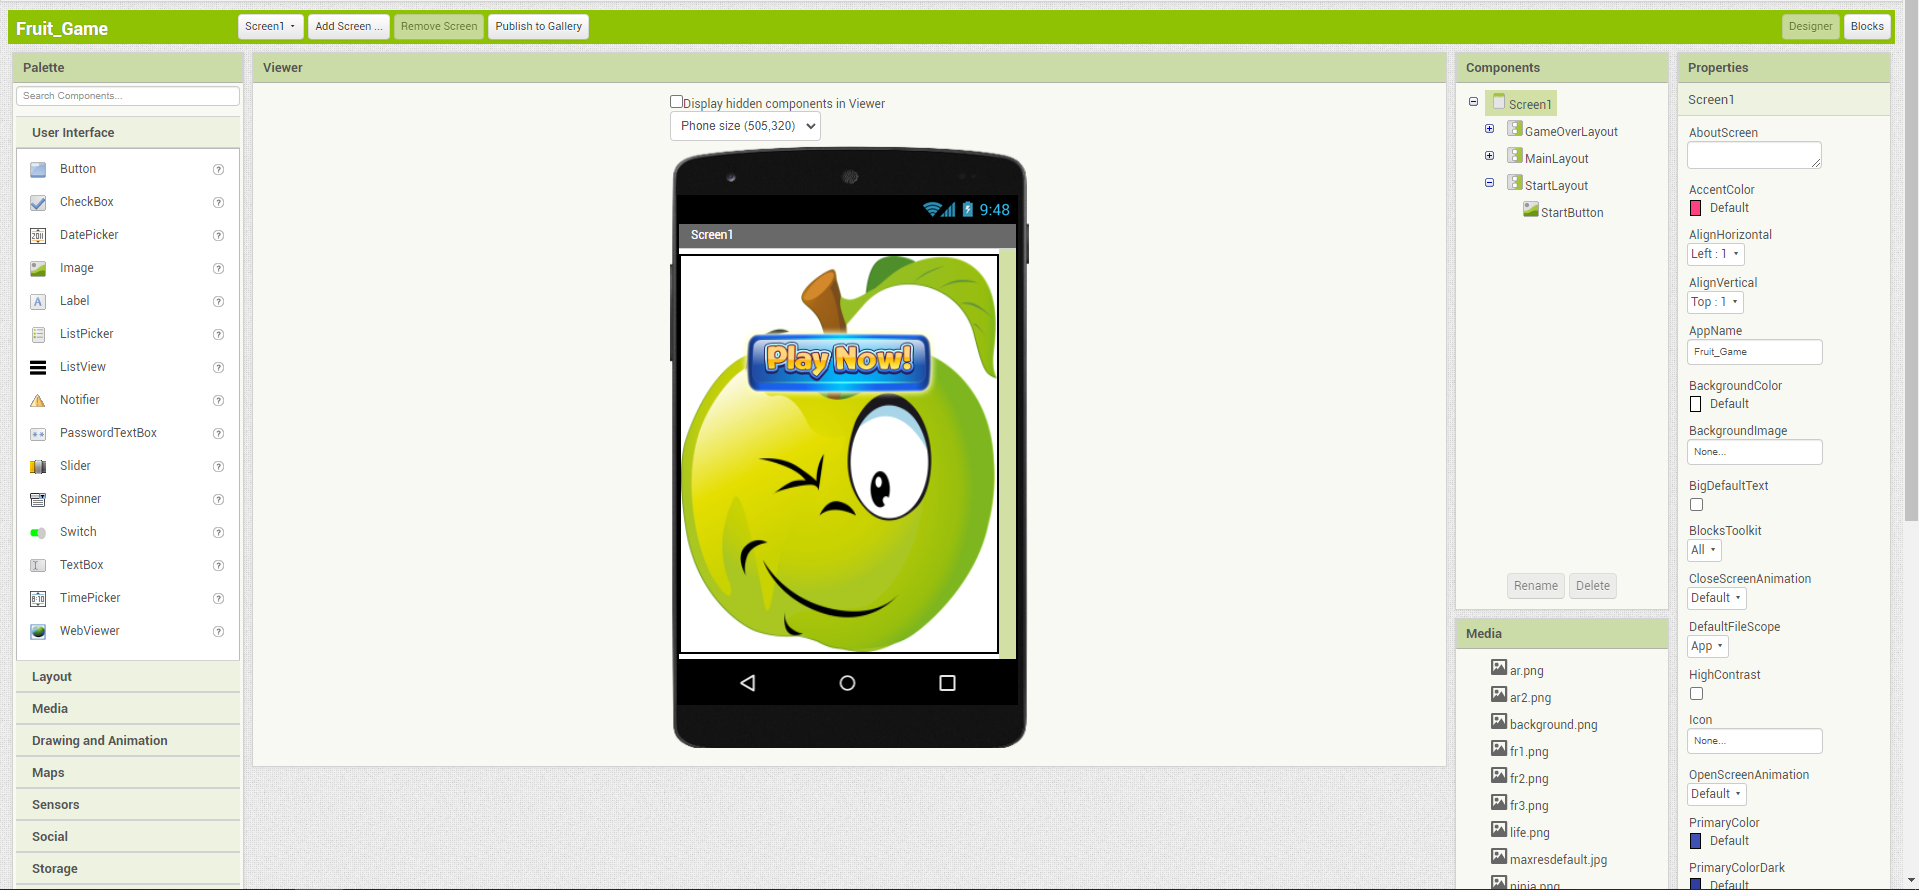
\includegraphics[width=1.0\linewidth,height=0.5\linewidth]{fig120001.png}
   \caption{Collect the fruits}
\label{fig120001}
\end{figure}

\section{Creating the Design}
Building the game starts with creating the design and what the game will look like. The first step is to add a Layout to be a VerticalArrangement. It is required for the splash screen when the game starts. The dimensions of this element should be as they are on the phone screen. For this, the height and width properties must be changed.

\begin{figure}[H]
   \centering
   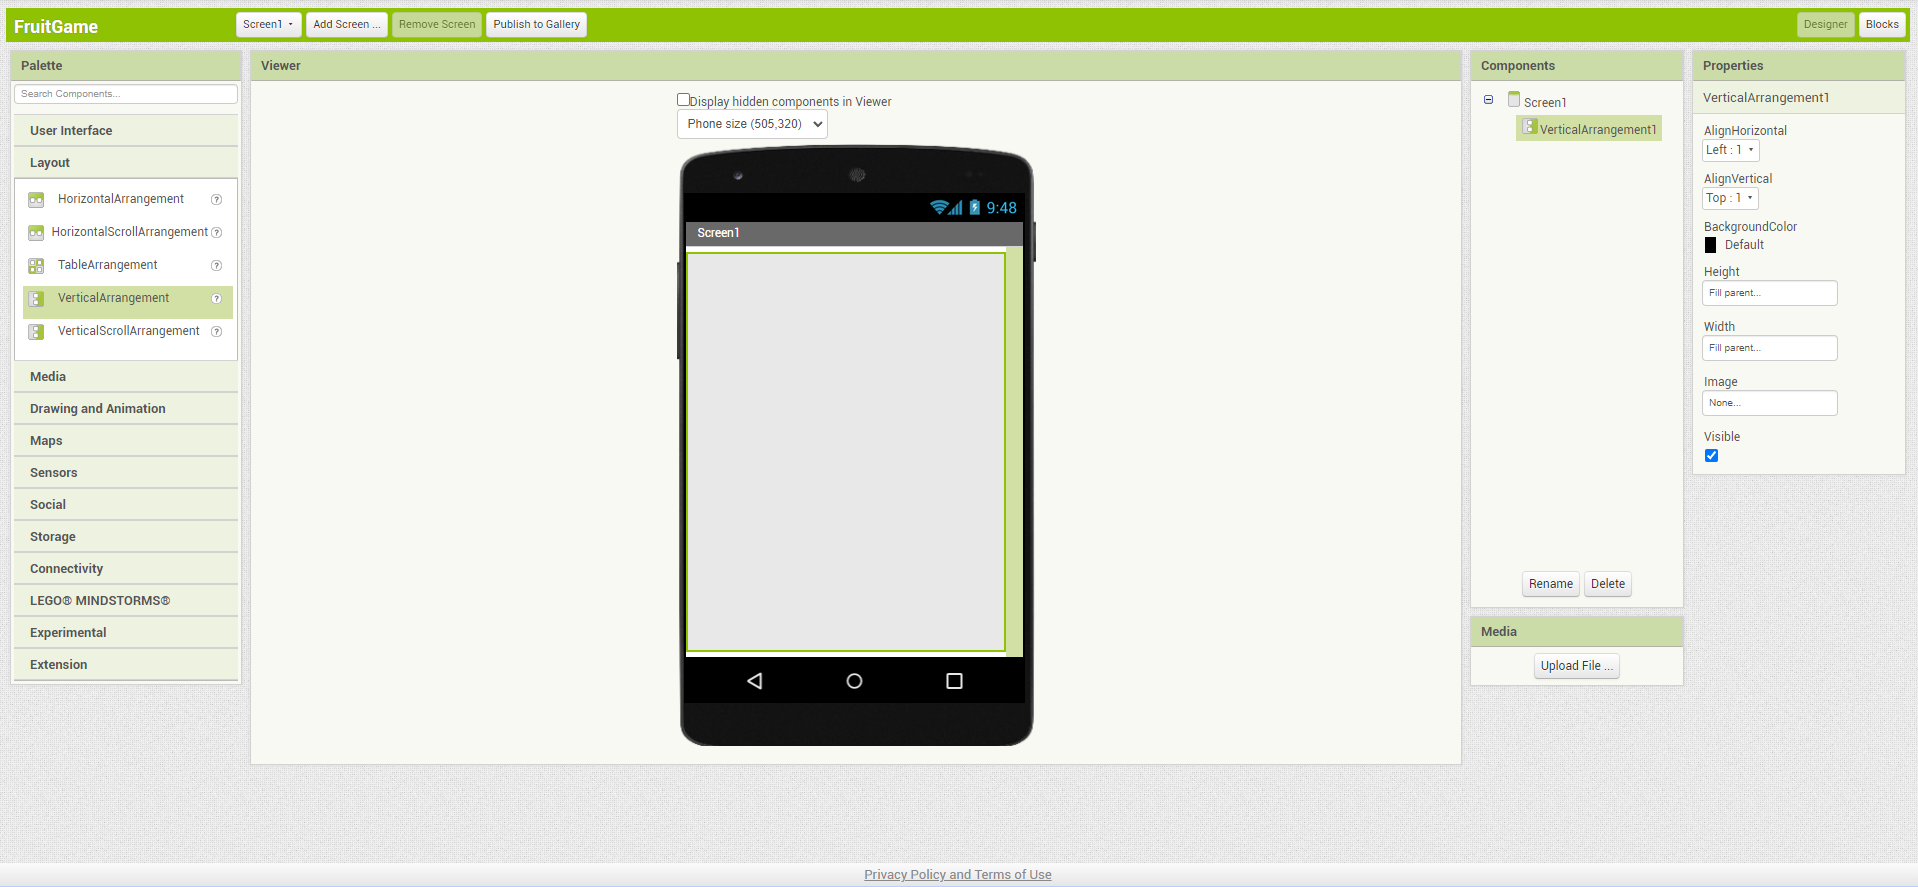
\includegraphics[width=1.0\linewidth,height=0.5\linewidth]{fig120002.png}
   \caption{Home Screen}
\label{fig120002}
\end{figure}

To make the beginning more attractive, an image can be added. All images shown in this example can be replaced. Any images distributed under a free license may be used.

When the game starts, the selected image should be added to the Image property to be displayed on the phone screen.

\begin{figure}[H]
   \centering
   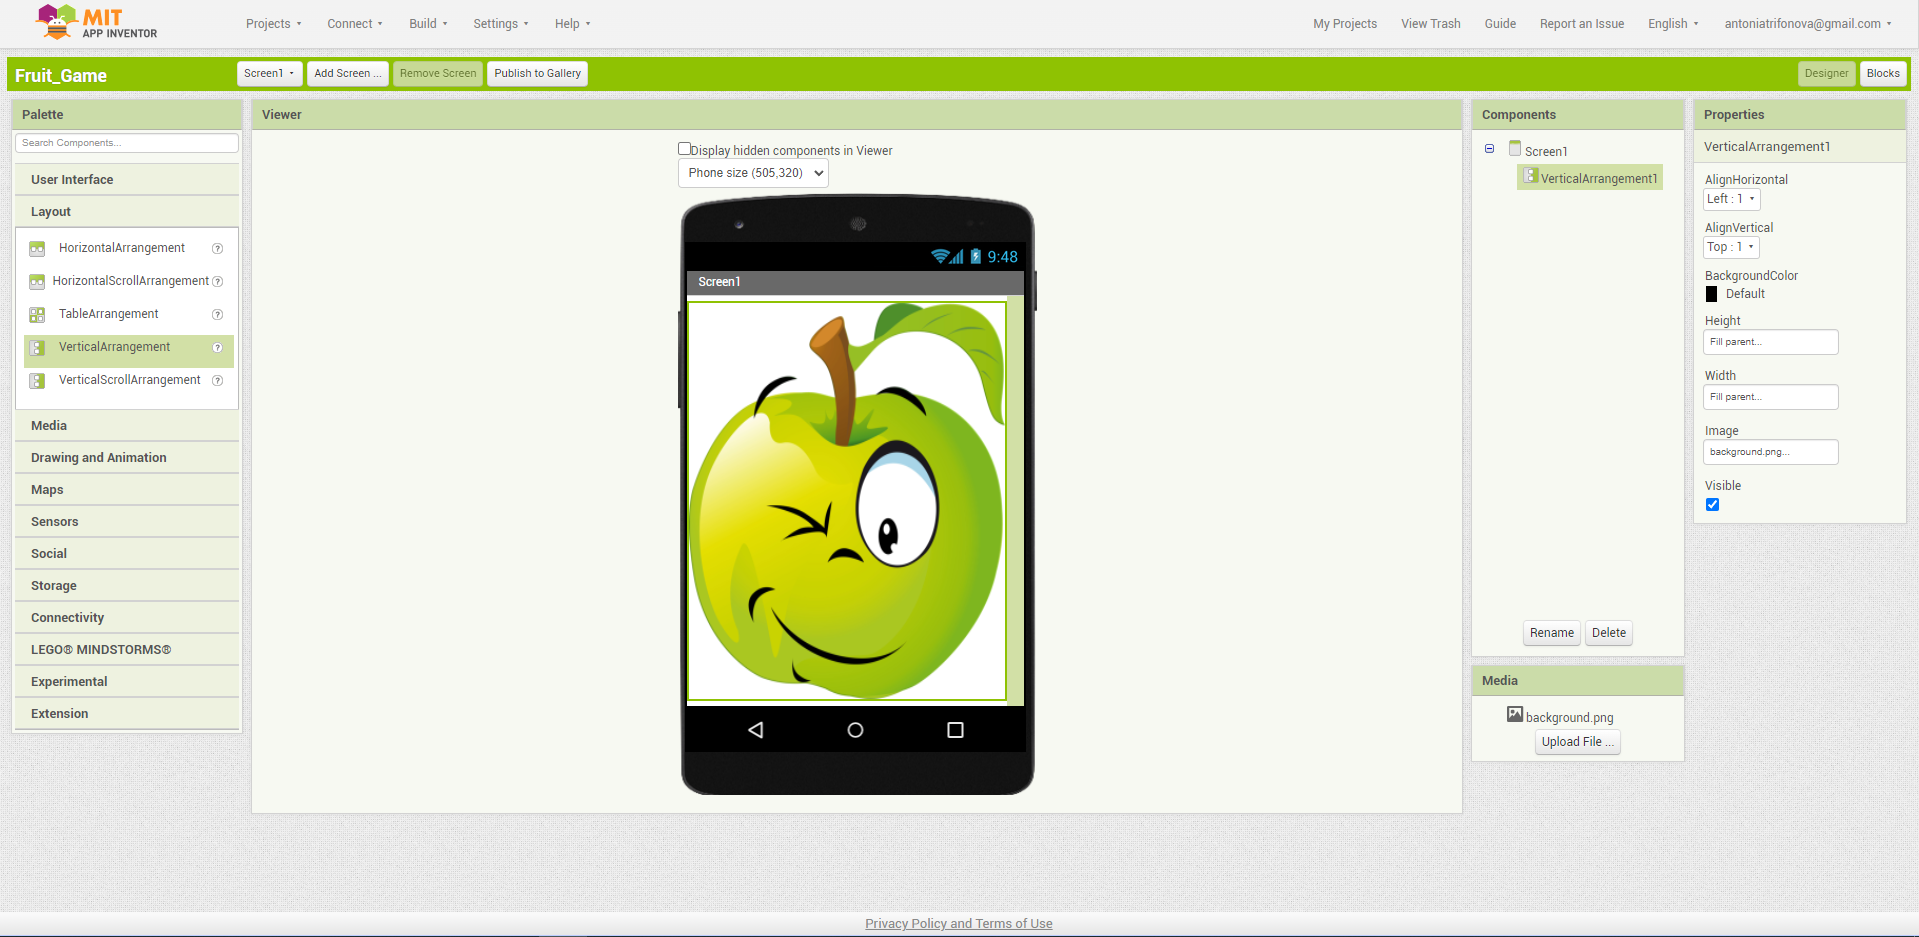
\includegraphics[width=1.0\linewidth,height=0.5\linewidth]{fig120003.png}
   \caption{Home Screen Background}
\label{fig120003}
\end{figure}

The game will start when the player presses the start button. A button element should also be added for this purpose. It is possible to use the built-in button element, but the Image element can be used to make the game more attractive. An image can be used for the button. It is essential to highlight the Clickable property. The Height and Width properties are responsible for how tall and wide the image should be.

\begin{figure}[H]
   \centering
   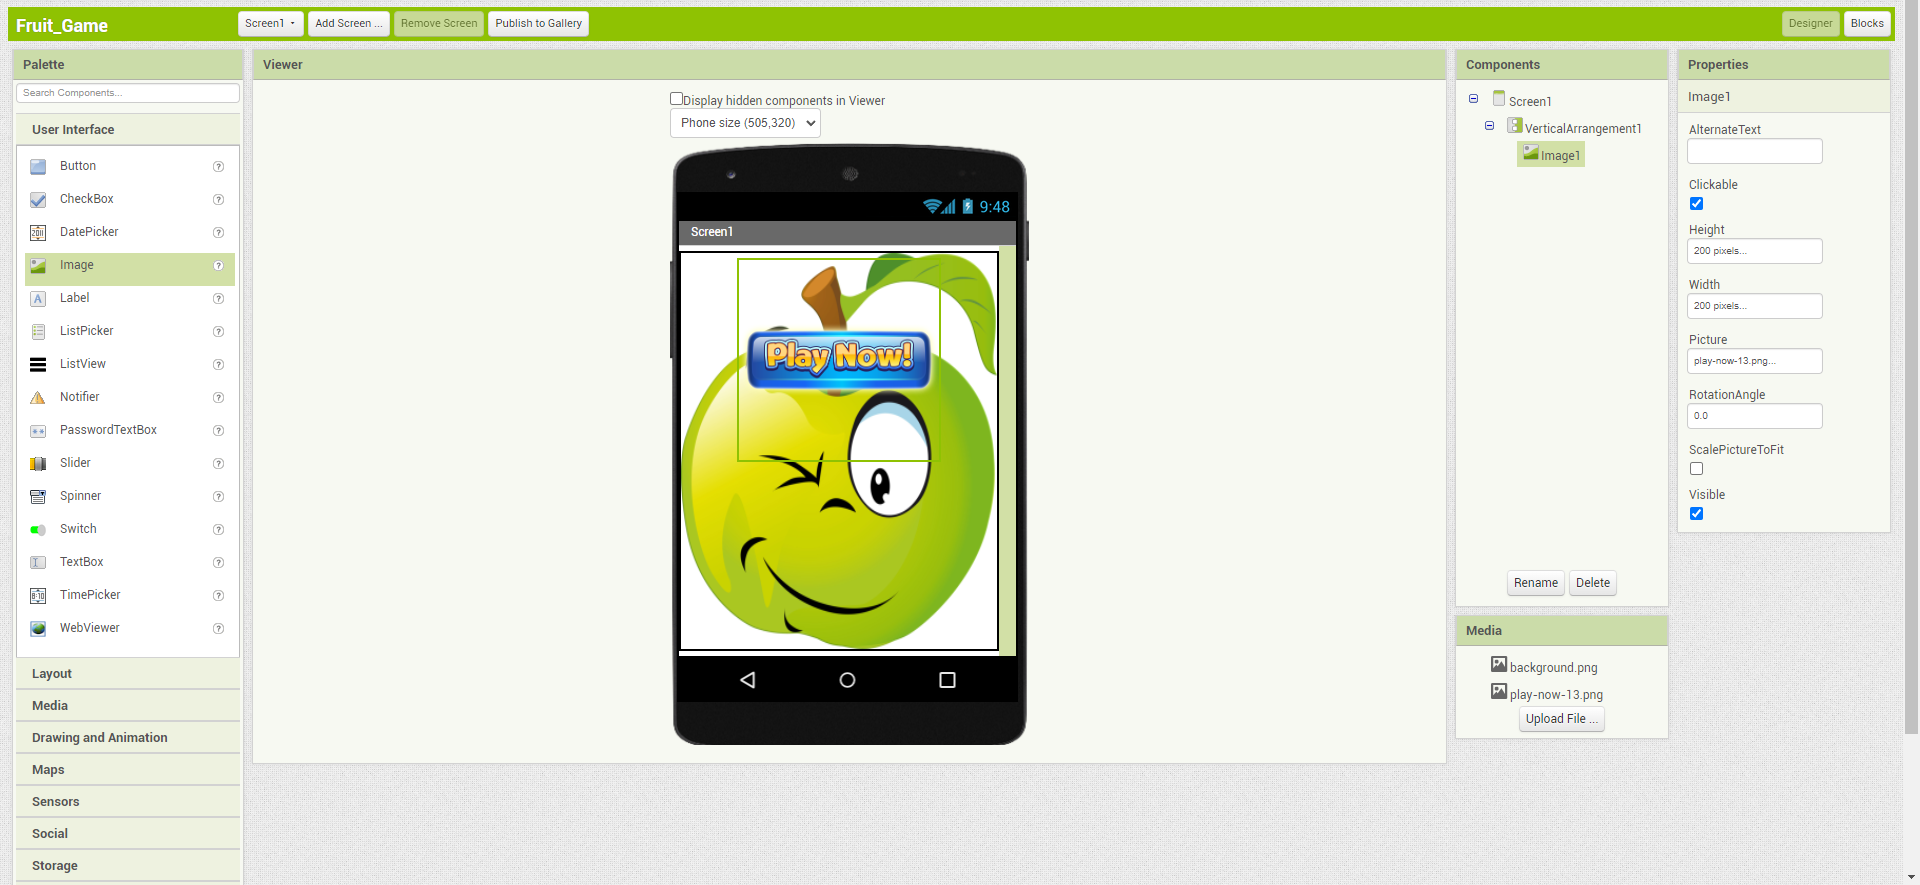
\includegraphics[width=1.0\linewidth,height=0.5\linewidth]{fig120004.png}
   \caption{Start Button}
\label{fig120004}
\end{figure}

When the game starts, this view will appear. When the player presses the button, another view should appear where the character is to be controlled, and the falling fruits will appear. To distinguish different game views when programming, it is good practice to have descriptive names. The VerticalArrangement1 element will be named StartLayout, and the Image1 element will be named StartButton.

\begin{figure}[H]
   \centering
   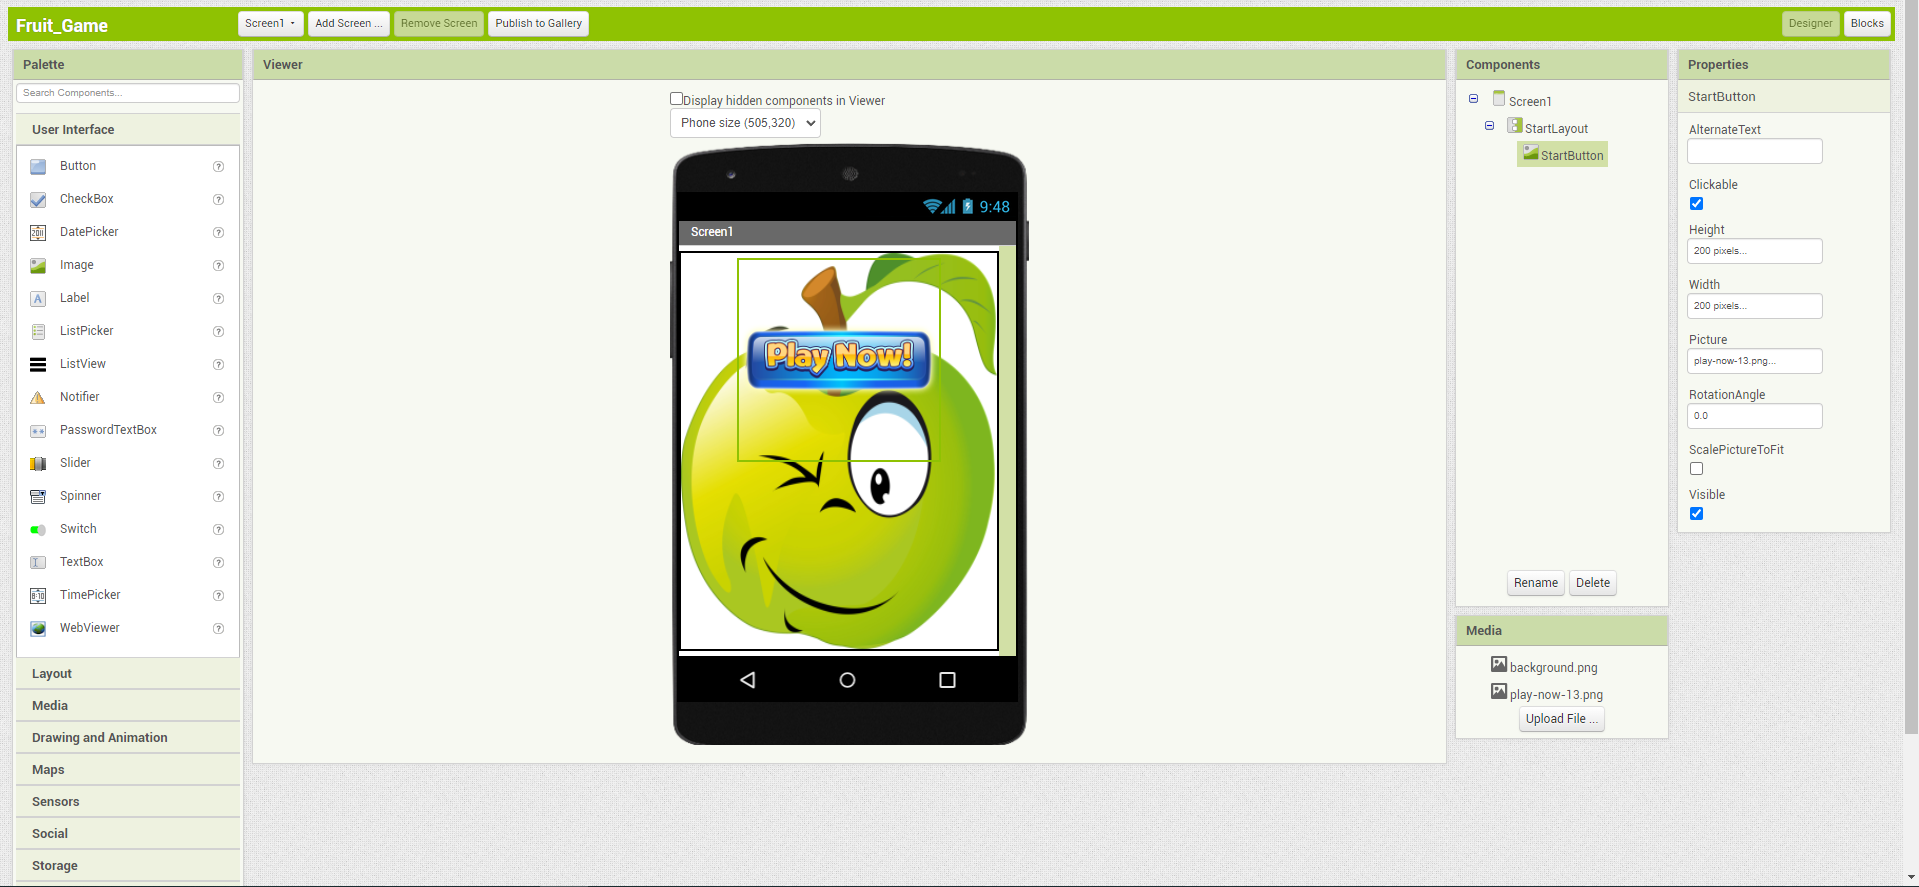
\includegraphics[width=1.0\linewidth,height=0.5\linewidth]{fig120005.png}
   \caption{Final version of splash screen}
\label{fig120005}
\end{figure}

To create the other view, a VerticalArrangement element called MainLayout must be added again. The height and width of this element must be the same as they are on the screen. To make this view's design more effortless, the StartLayout element's Visible property should be unchecked.

\begin{figure}[H]
   \centering
   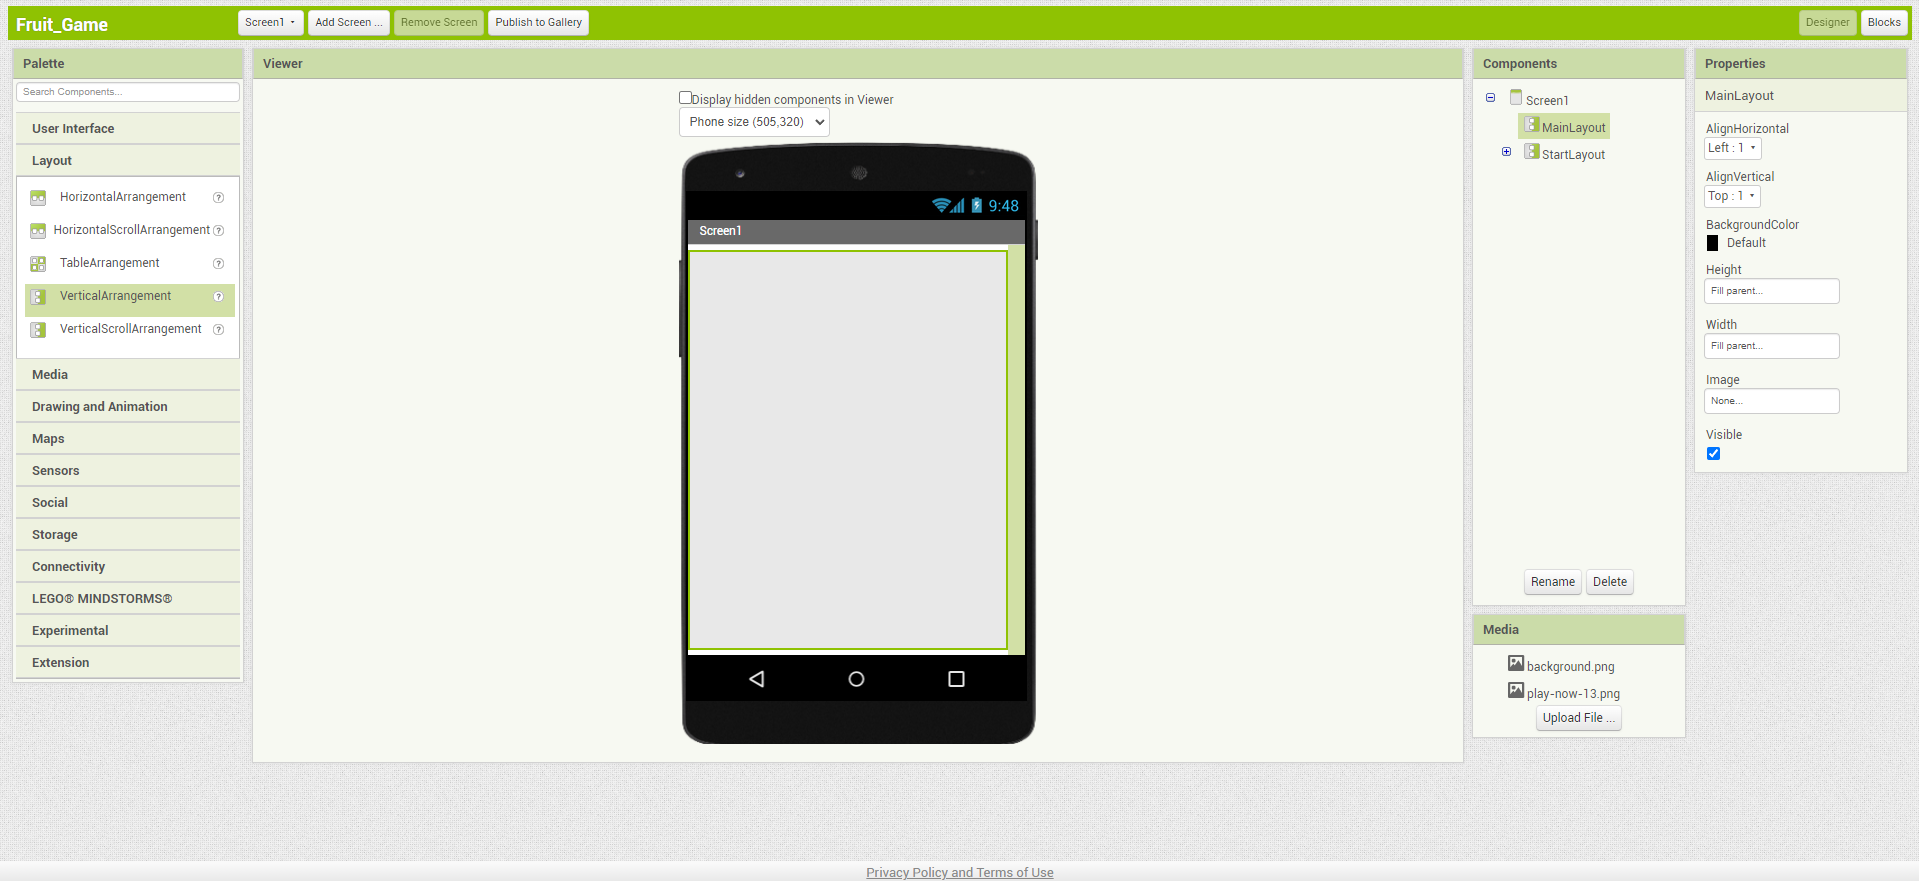
\includegraphics[width=1.0\linewidth,height=0.5\linewidth]{fig120006.png}
   \caption{Creating main game screen}
\label{fig120006}
\end{figure}

The Canvas and HorizontalArrangement elements should be added to the MainLayout element.
The Canvas element is necessary because it allows the elements inside it to move. Several items in the game will move. On the one hand, the character will catch the fruits, and on the other, the fruits themselves.
The height and width of this element must be the same as they are on the screen. Again, a background can also be added to this element.

\begin{figure}[H]
   \centering
   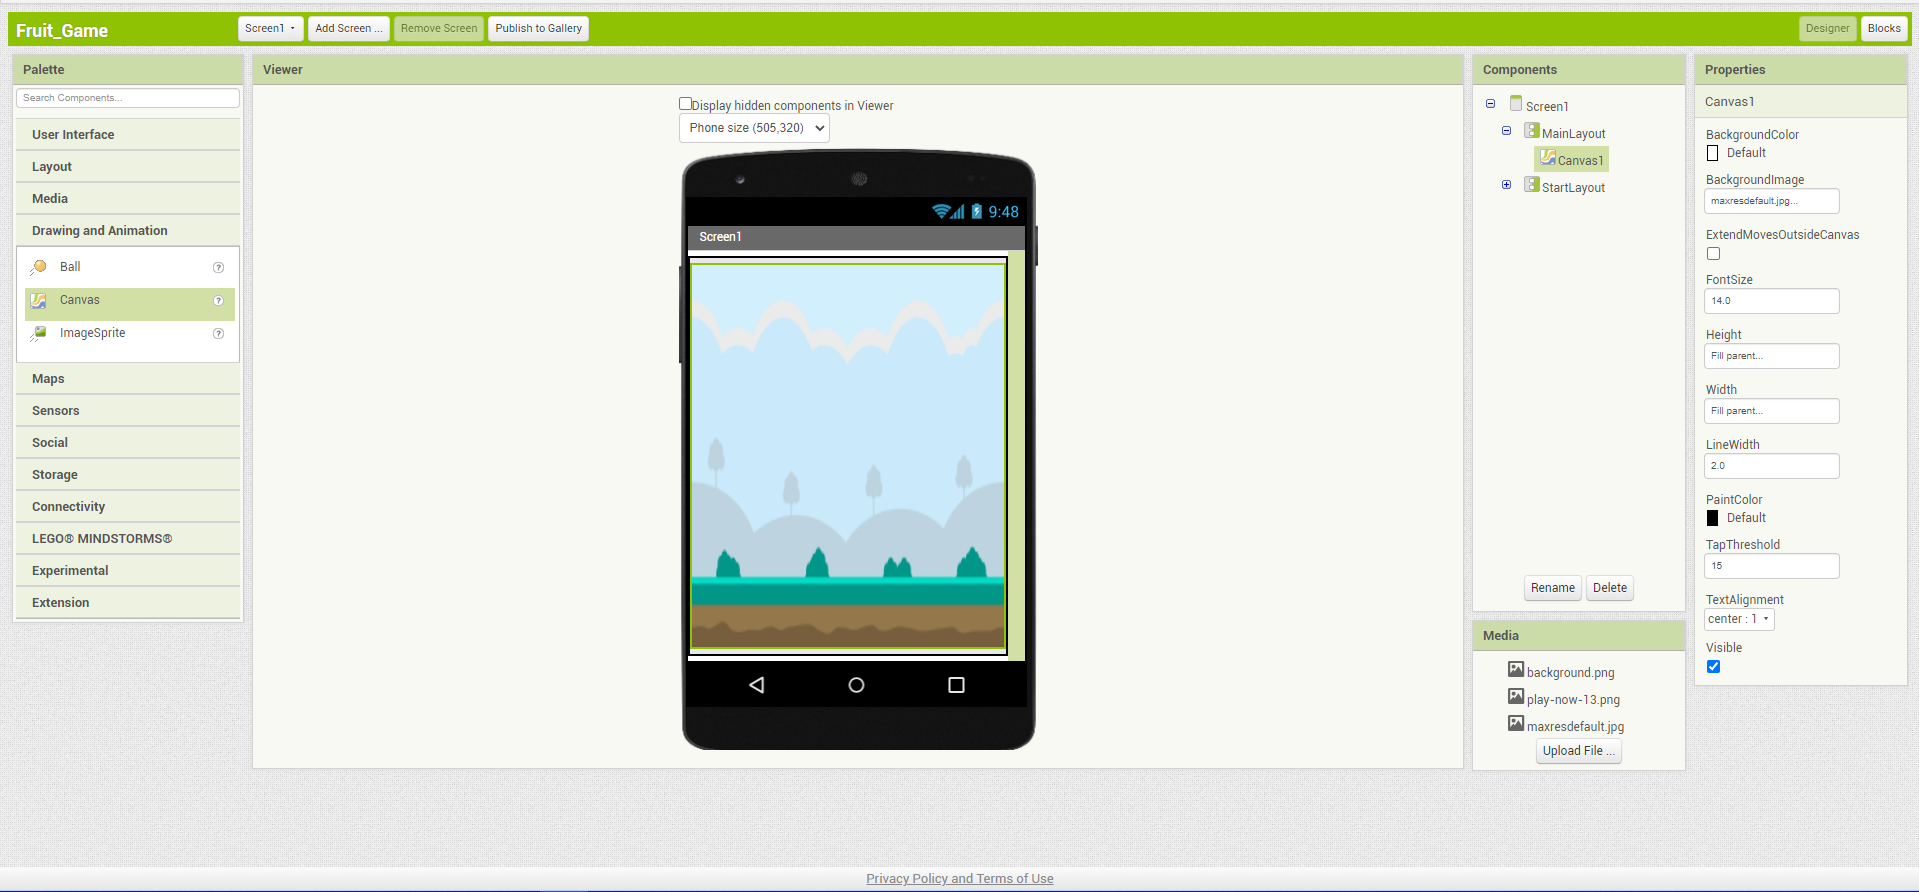
\includegraphics[width=1.0\linewidth,height=0.5\linewidth]{fig120007.png}
   \caption{Adding background to main game screen}
\label{fig120007}
\end{figure}

Several fruit images should be added to this element. Also, an image to be the character and three to be his life. Changing the Height and Width properties can change their sizes, and changing the X, Y, and Z properties can change their position. It is also essential to change the names of the elements so that they can be recognized when it comes to programming them.
The figure shows an example arrangement of the fruits, the character, and his life. For the purposes of the game, the number of fruits or their placement is irrelevant.

\begin{figure}[H]
   \centering
   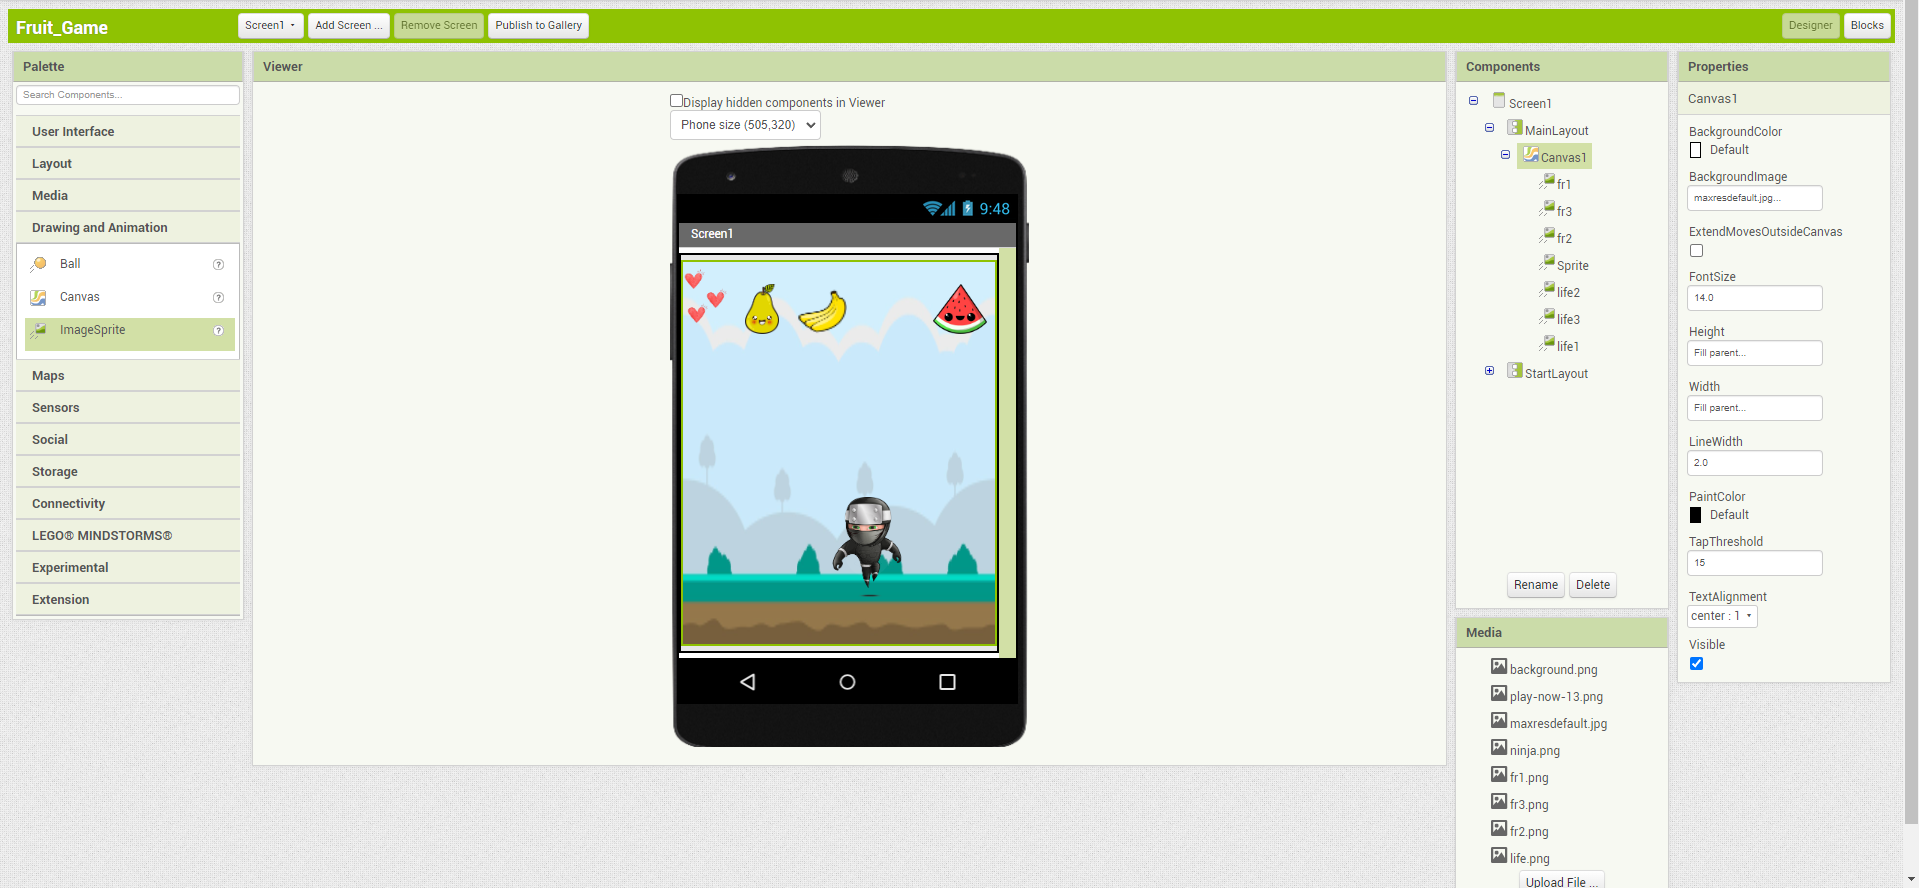
\includegraphics[width=1.0\linewidth,height=0.5\linewidth]{fig120008.png}
   \caption{Adding the fruits, lives, and character to the game}
\label{fig120008}
\end{figure}

A HorizontalArrangement element must be added to complete this view, to which the two buttons - left arrow and right arrow - will be added. These buttons will control the player to move. A Label element can be placed between them, showing how many points the player has earned.
The width of the HorizontalArrangement element should be the width of the screen. Its height should be small, for example, 10 percent. The AlignHorizontal and AlignVertical properties must be changed to Center for the elements inside to align.

\begin{figure}[H]
   \centering
   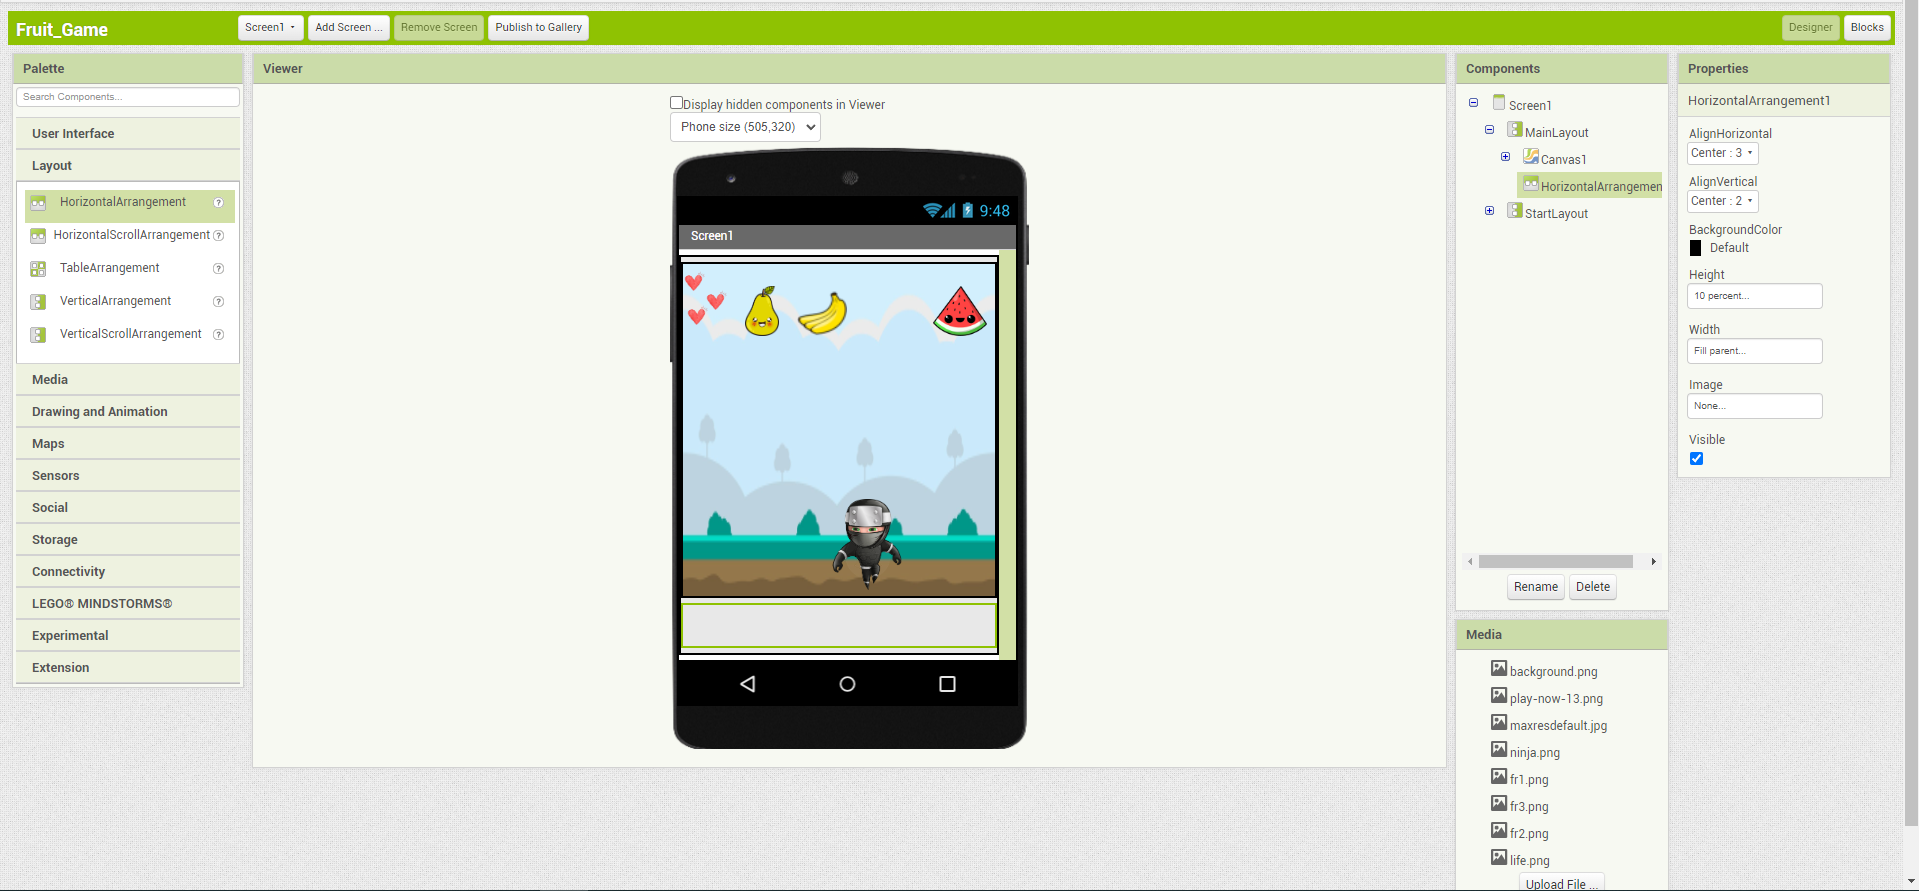
\includegraphics[width=1.0\linewidth,height=0.5\linewidth]{fig120009.png}
   \caption{Add control bar}
\label{fig120009}
\end{figure}

The buttons should be added by resizing them and adding images to look like left and right arrows.

\begin{figure}[H]
   \centering
   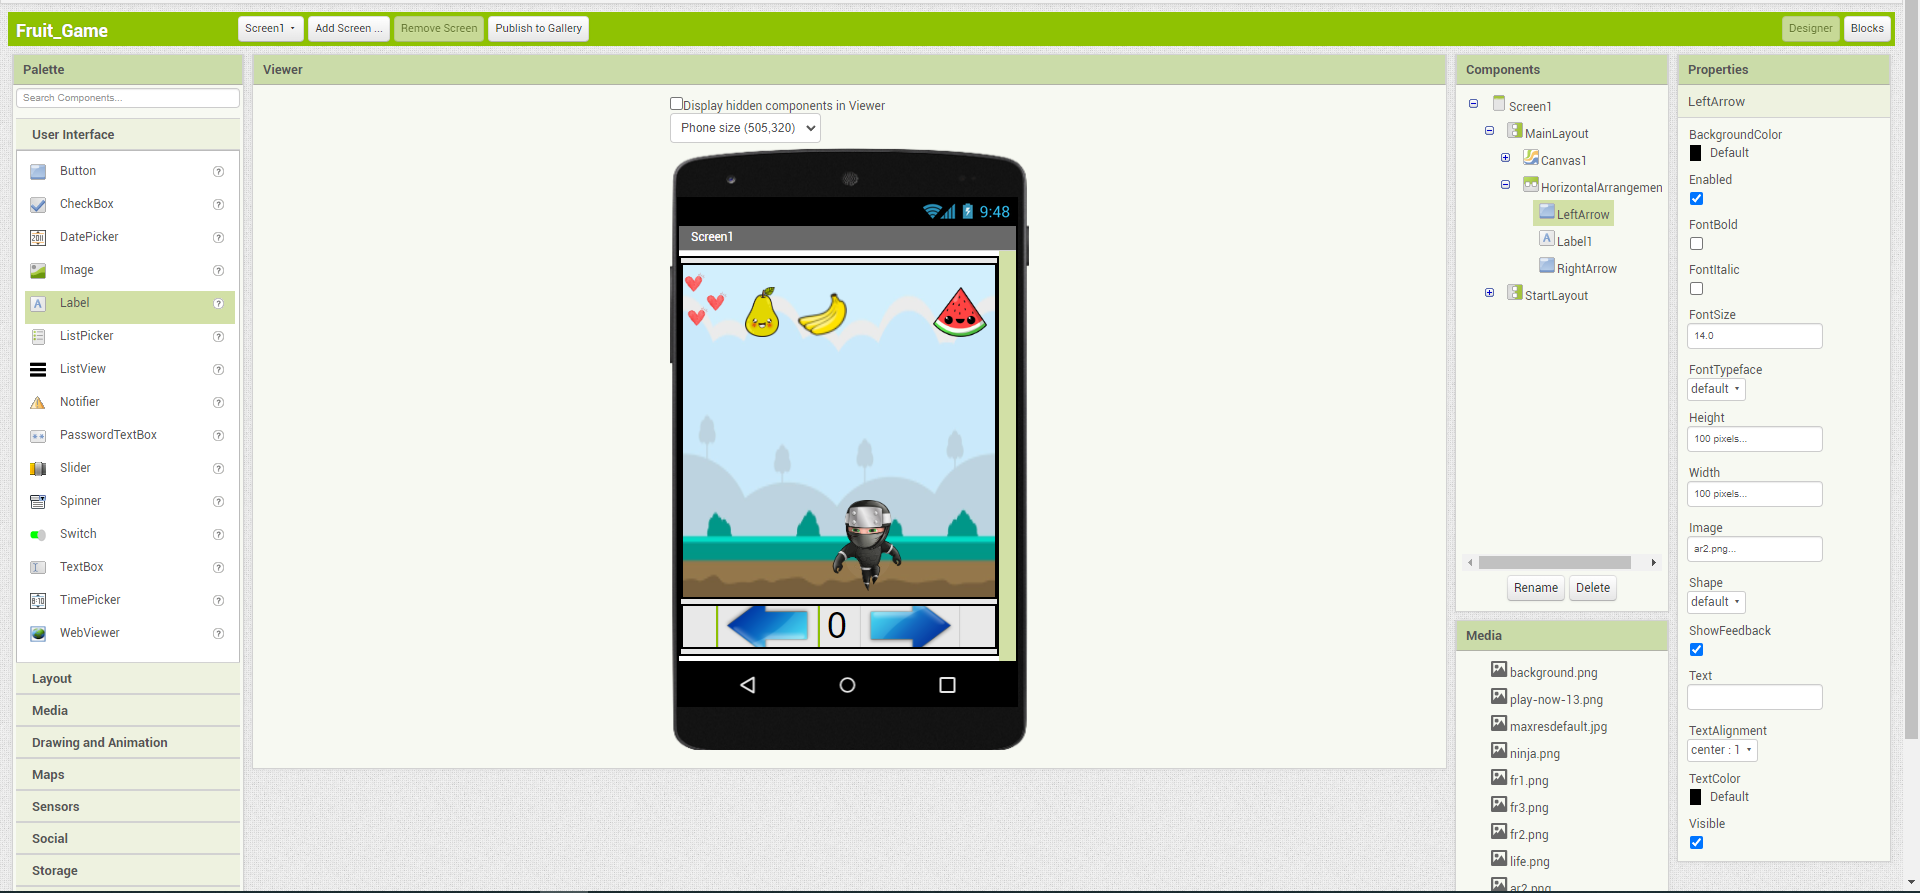
\includegraphics[width=1.0\linewidth,height=0.5\linewidth]{fig120010.png}
   \caption{Adding the controls}
\label{fig120010}
\end{figure}

For the Label element, where the points will be written, the value of the FontSize property must be changed so that the text can be larger and more visible.

\begin{figure}[H]
   \centering
   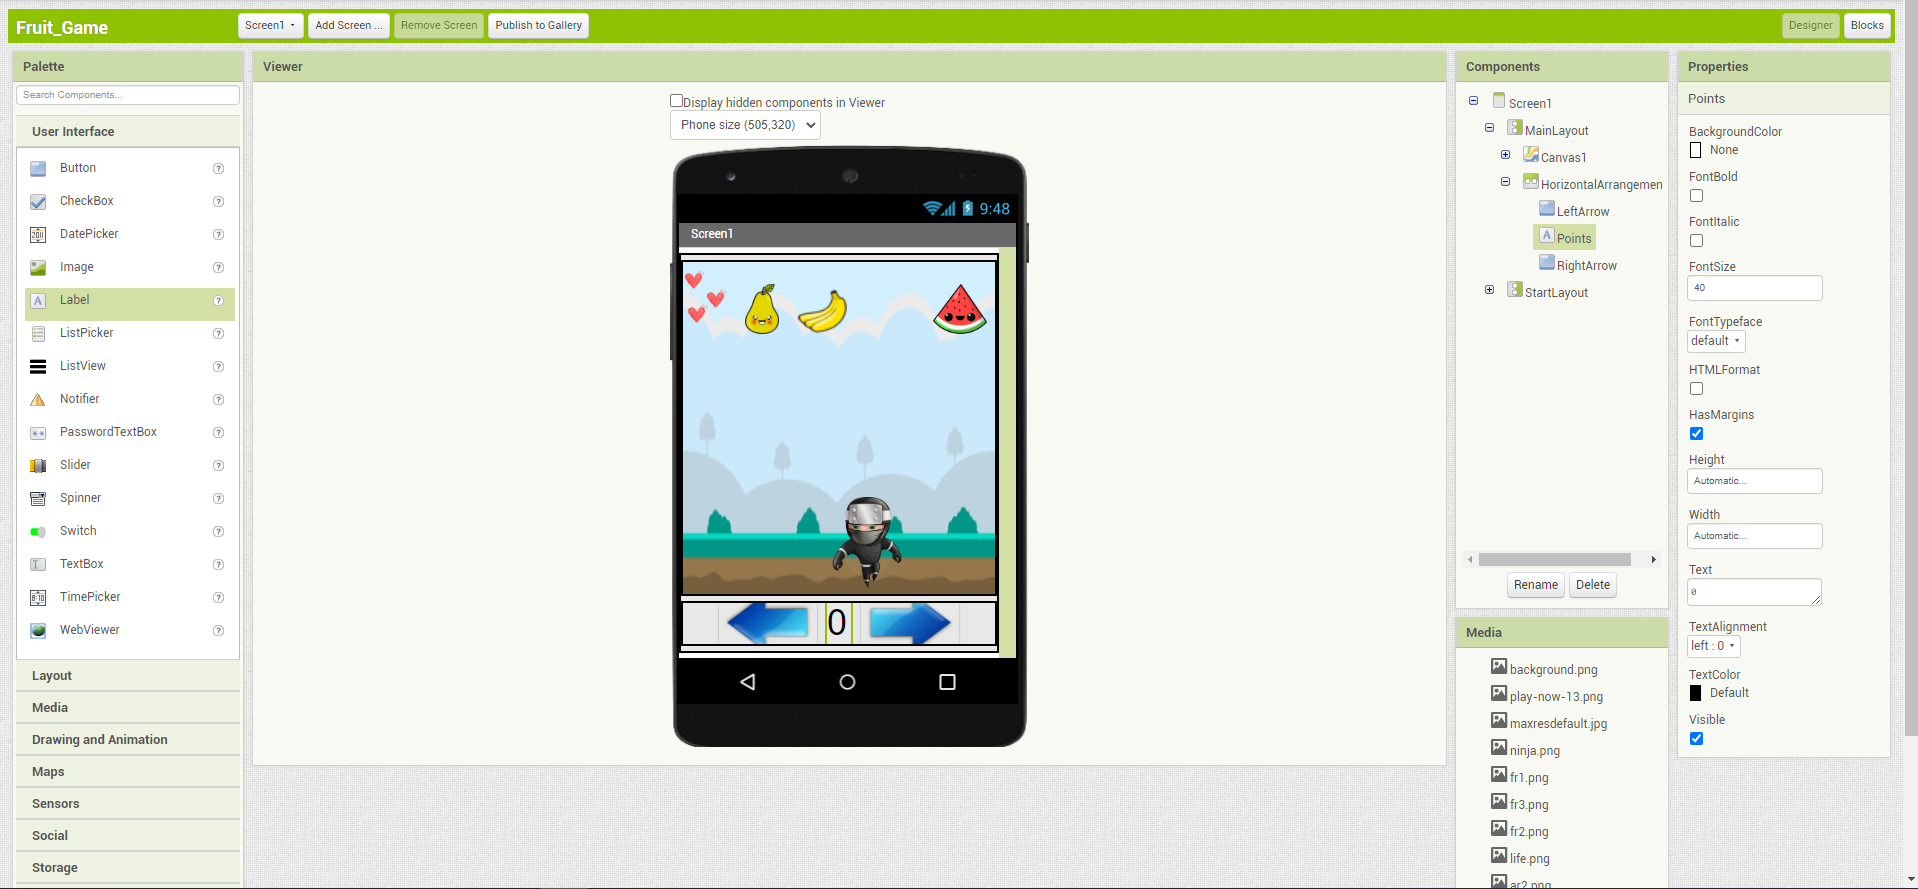
\includegraphics[width=1.0\linewidth,height=0.5\linewidth]{fig120011.png}
   \caption{Change point size}
\label{fig120011}
\end{figure}

The last view to be designed is when the player loses their lives. Then a "Try again" button should be displayed. To make the design more straightforward, the Visible property of the MainLayout element must be unchecked.

\begin{figure}[H]
   \centering
   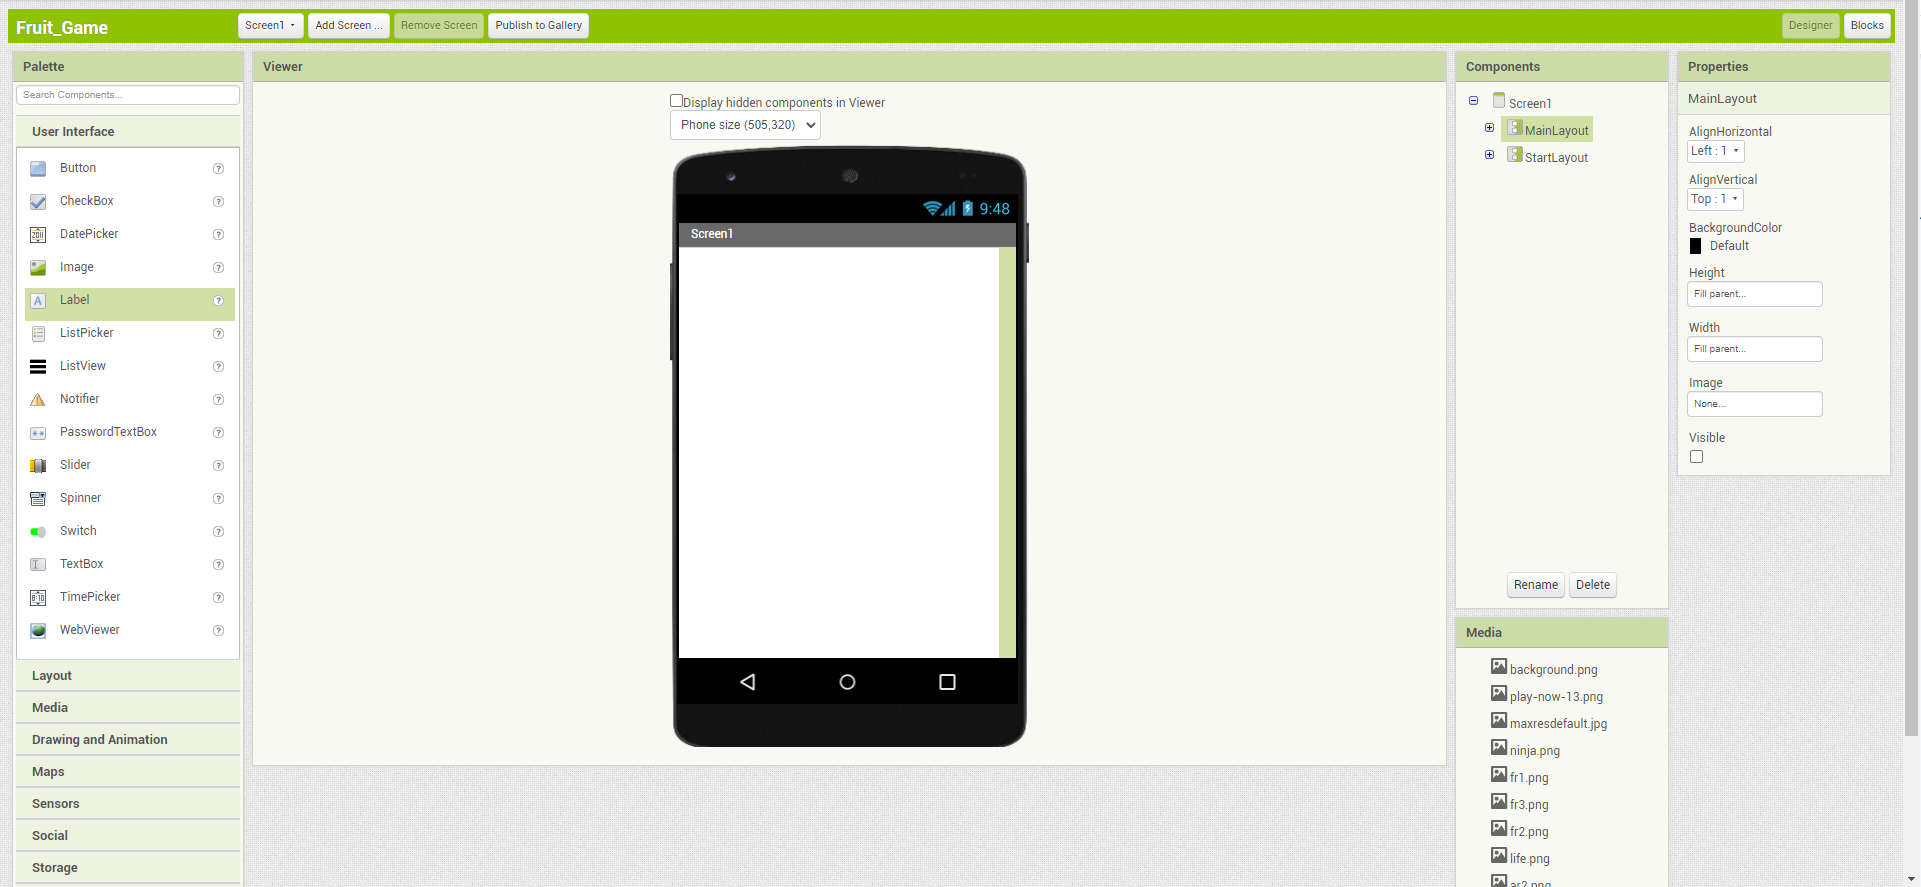
\includegraphics[width=1.0\linewidth,height=0.5\linewidth]{fig120012.png}
   \caption{Add end game view}
\label{fig120012}
\end{figure}

The view ending the game should be HorizontalArrangement again, with the height and width dimensions being the same on the screen. The background color of this element can be changed, or an endgame image can be added. The AlignHorizontal and AlignVertical property values must be set to Center for the game restart button to be centered.

\begin{figure}[H]
   \centering
   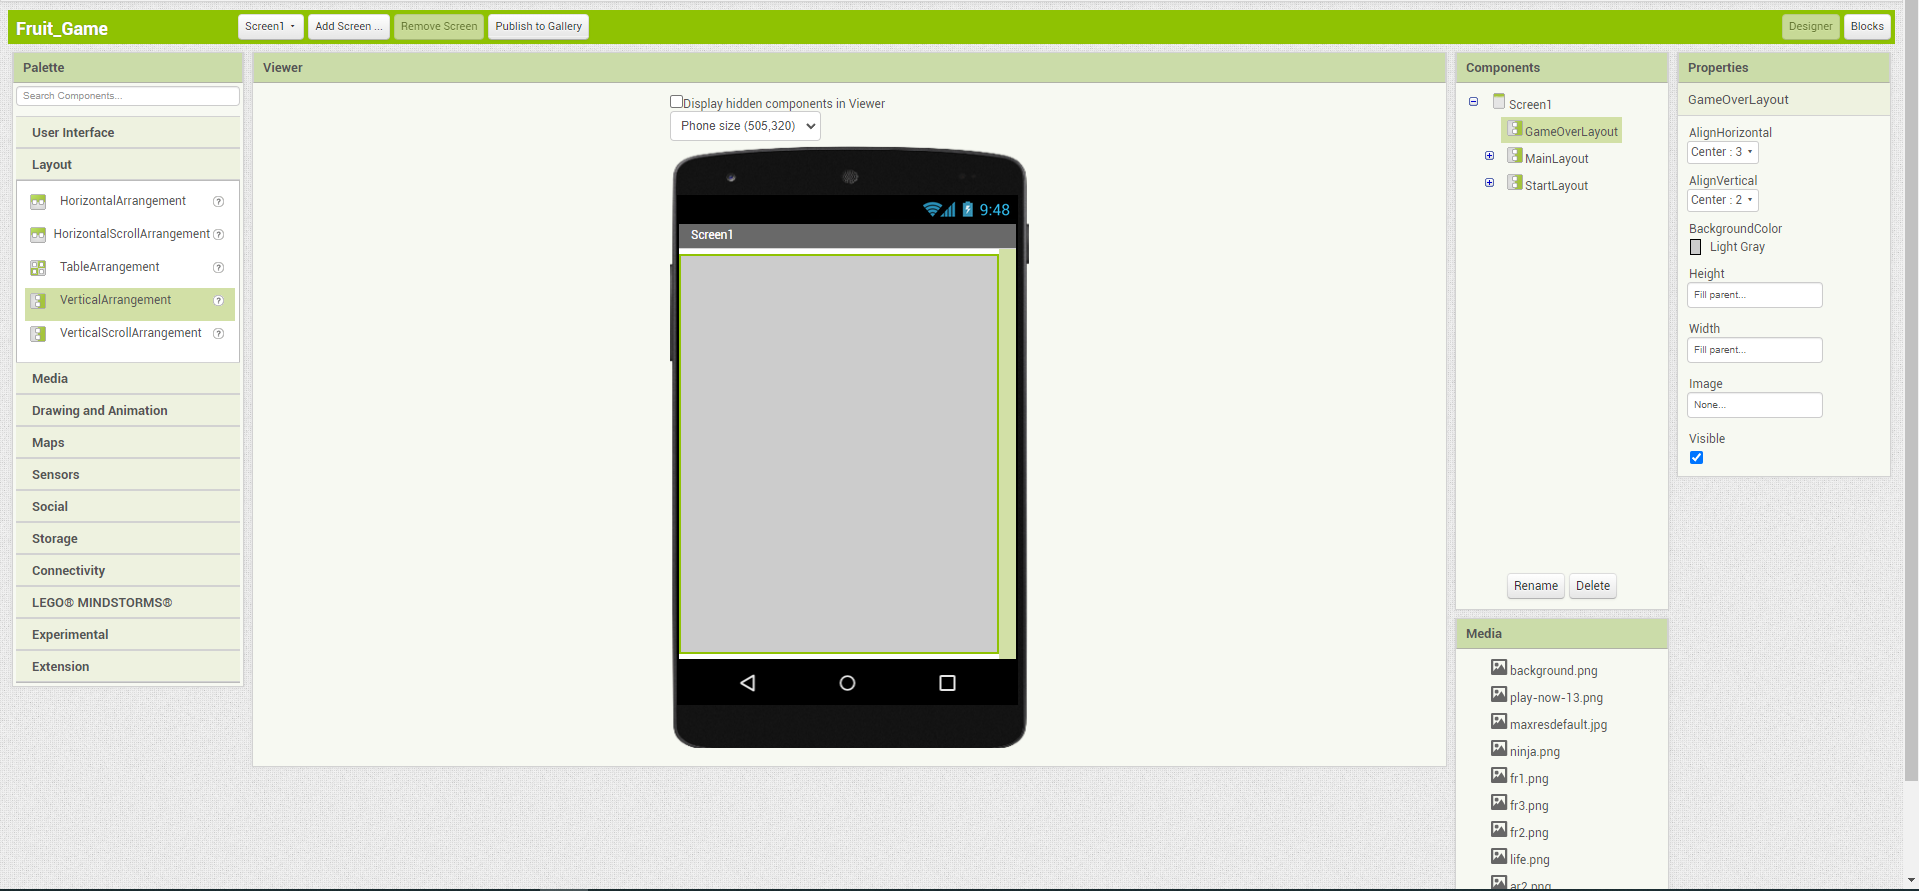
\includegraphics[width=1.0\linewidth,height=0.5\linewidth]{fig120013.png}
   \caption{Change background color}
\label{fig120013}
\end{figure}

Lastly, the game restart button should be added. The button's shape, text size, and color properties can be changed.

\begin{figure}[H]
   \centering
   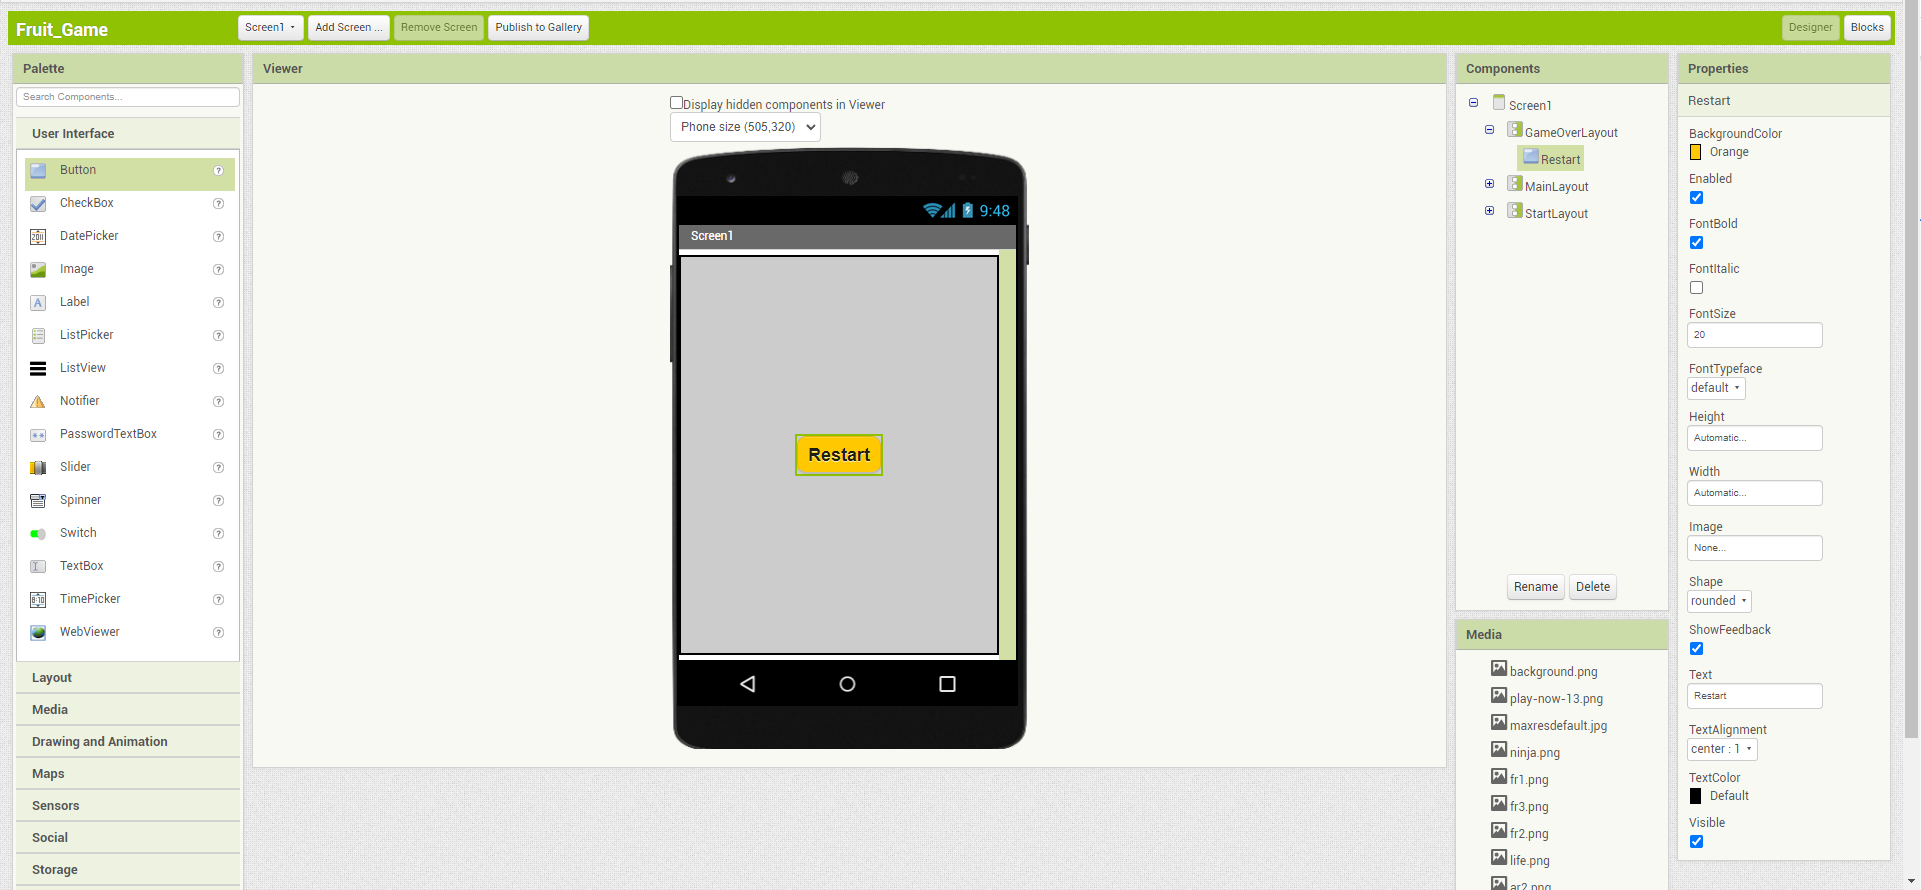
\includegraphics[width=1.0\linewidth,height=0.5\linewidth]{fig120014.png}
   \caption{Add game restart button}
\label{fig120014}
\end{figure}

The Visible property of the GameOverLayout element should be unchecked. Only the game start screen should be visible. For this, it must be marked for the StartLayout element.

\begin{figure}[H]
   \centering
   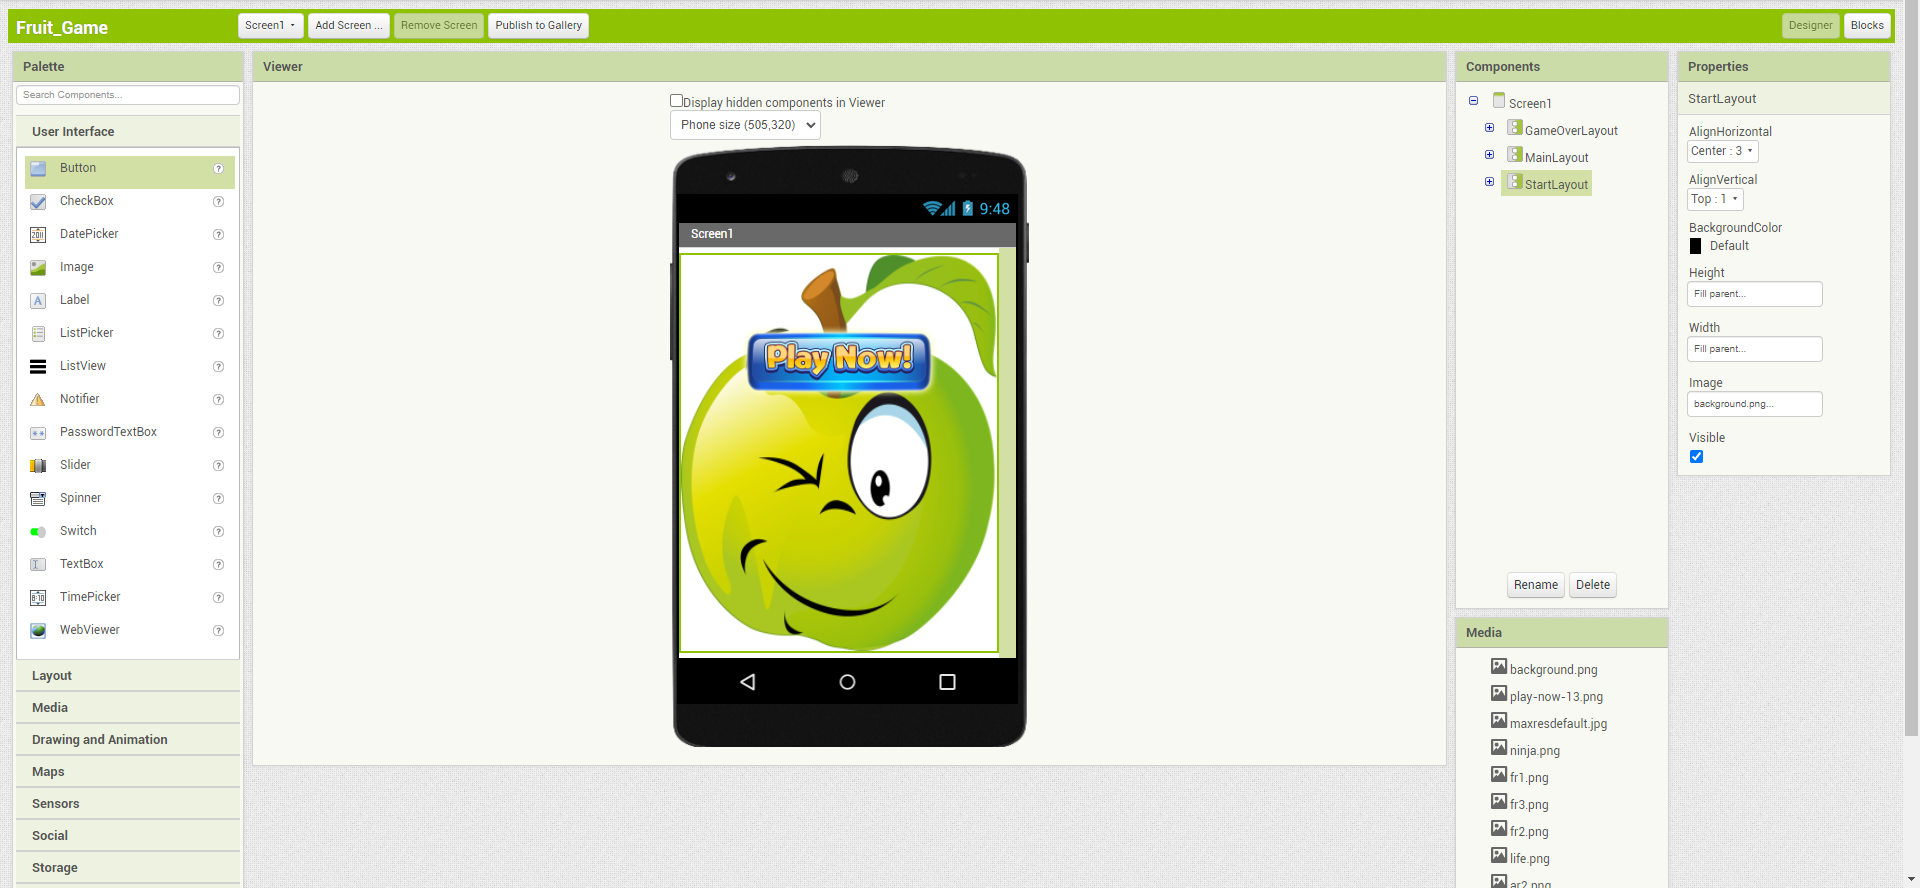
\includegraphics[width=1.0\linewidth,height=0.5\linewidth]{fig120015.png}
   \caption{Checking the Visible property for the home screen}
\label{fig120015}
\end{figure}

\section{Creating the Program}
Blocks called "procedures" will be used to construct the game code. A procedure is characterized by a name and a set of instructions. They are executed when it is called. The purpose of a procedure is to contain instructions that are repeated at some point in the code. The following steps explain where and why procedures need to be used.

The first procedure to create is to start the game. The instructions will be in it for the initial positions of the fruits and set the speeds at which they will move. This sequence of steps must be performed when the game starts, i.e., the player presses the start game button and presses the restart game button. A procedure is used to avoid constructing the same steps twice for this.

\begin{figure}[H]
   \centering
   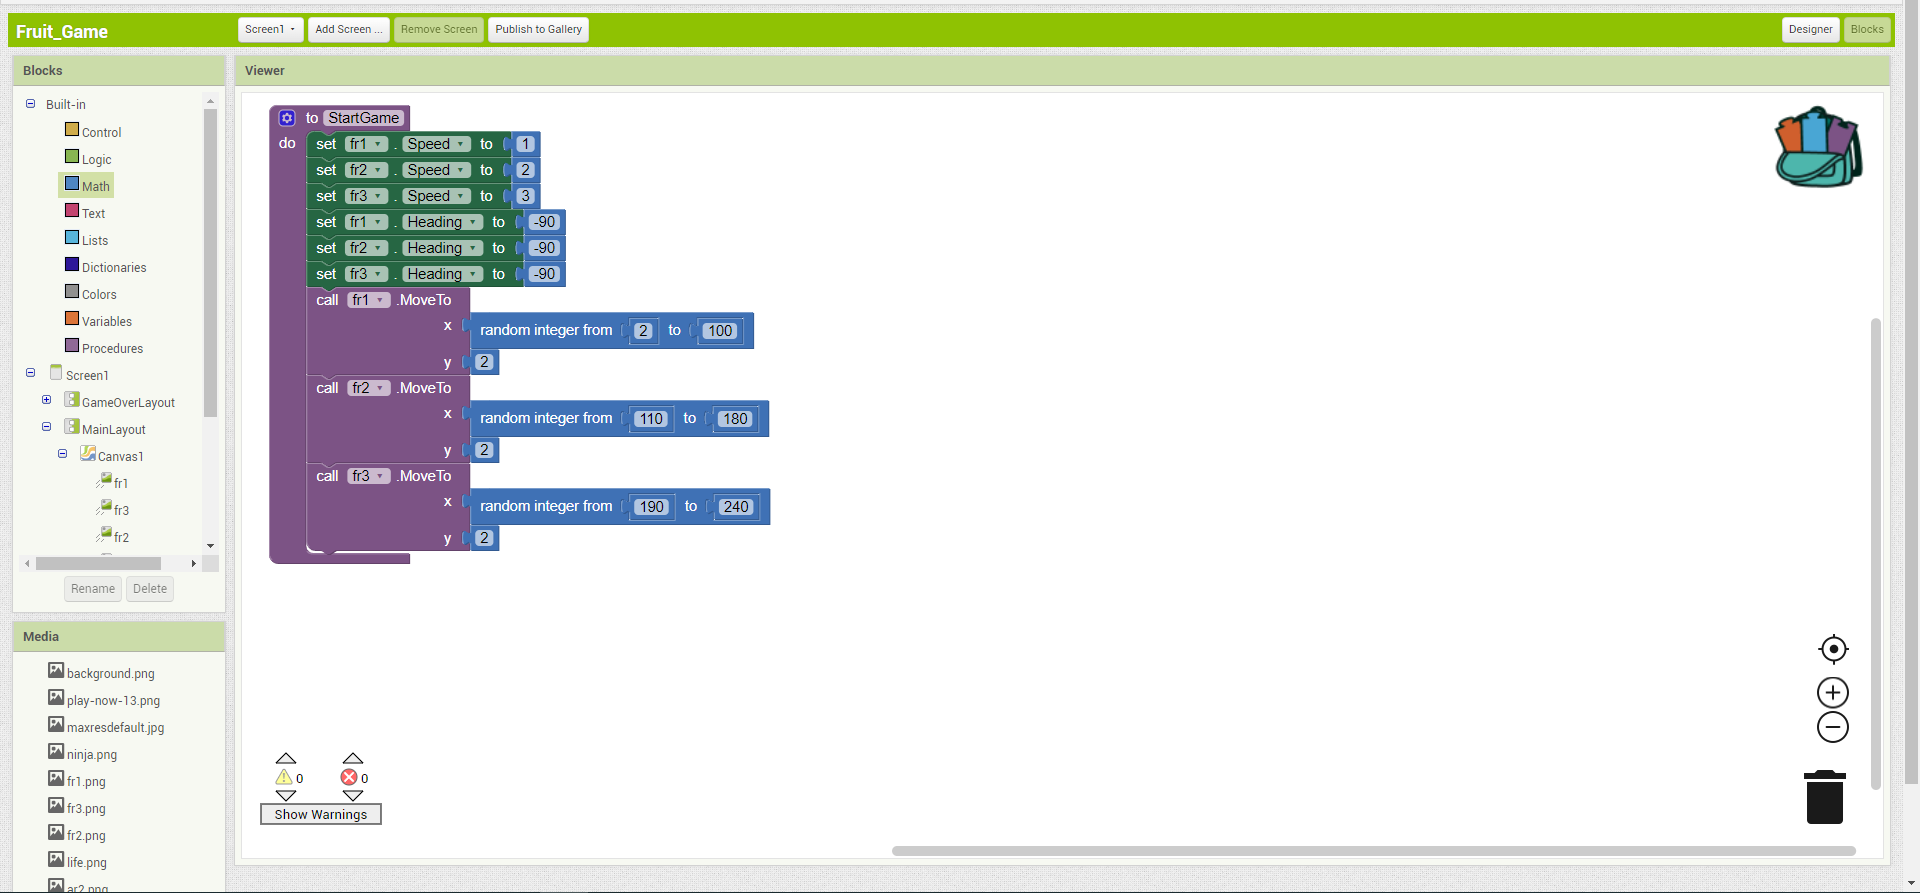
\includegraphics[width=1.0\linewidth,height=0.5\linewidth]{fig120016.png}
   \caption{Create Game Start Procedure}
\label{fig120016}
\end{figure}

This procedure will be first called when the StartButton is pressed. Besides calling the procedure, the other instructions to execute are to hide the start view and bring up the main view. This is implemented using the Visible property, which can be controlled through design and programmatically.

\begin{figure}[H]
   \centering
   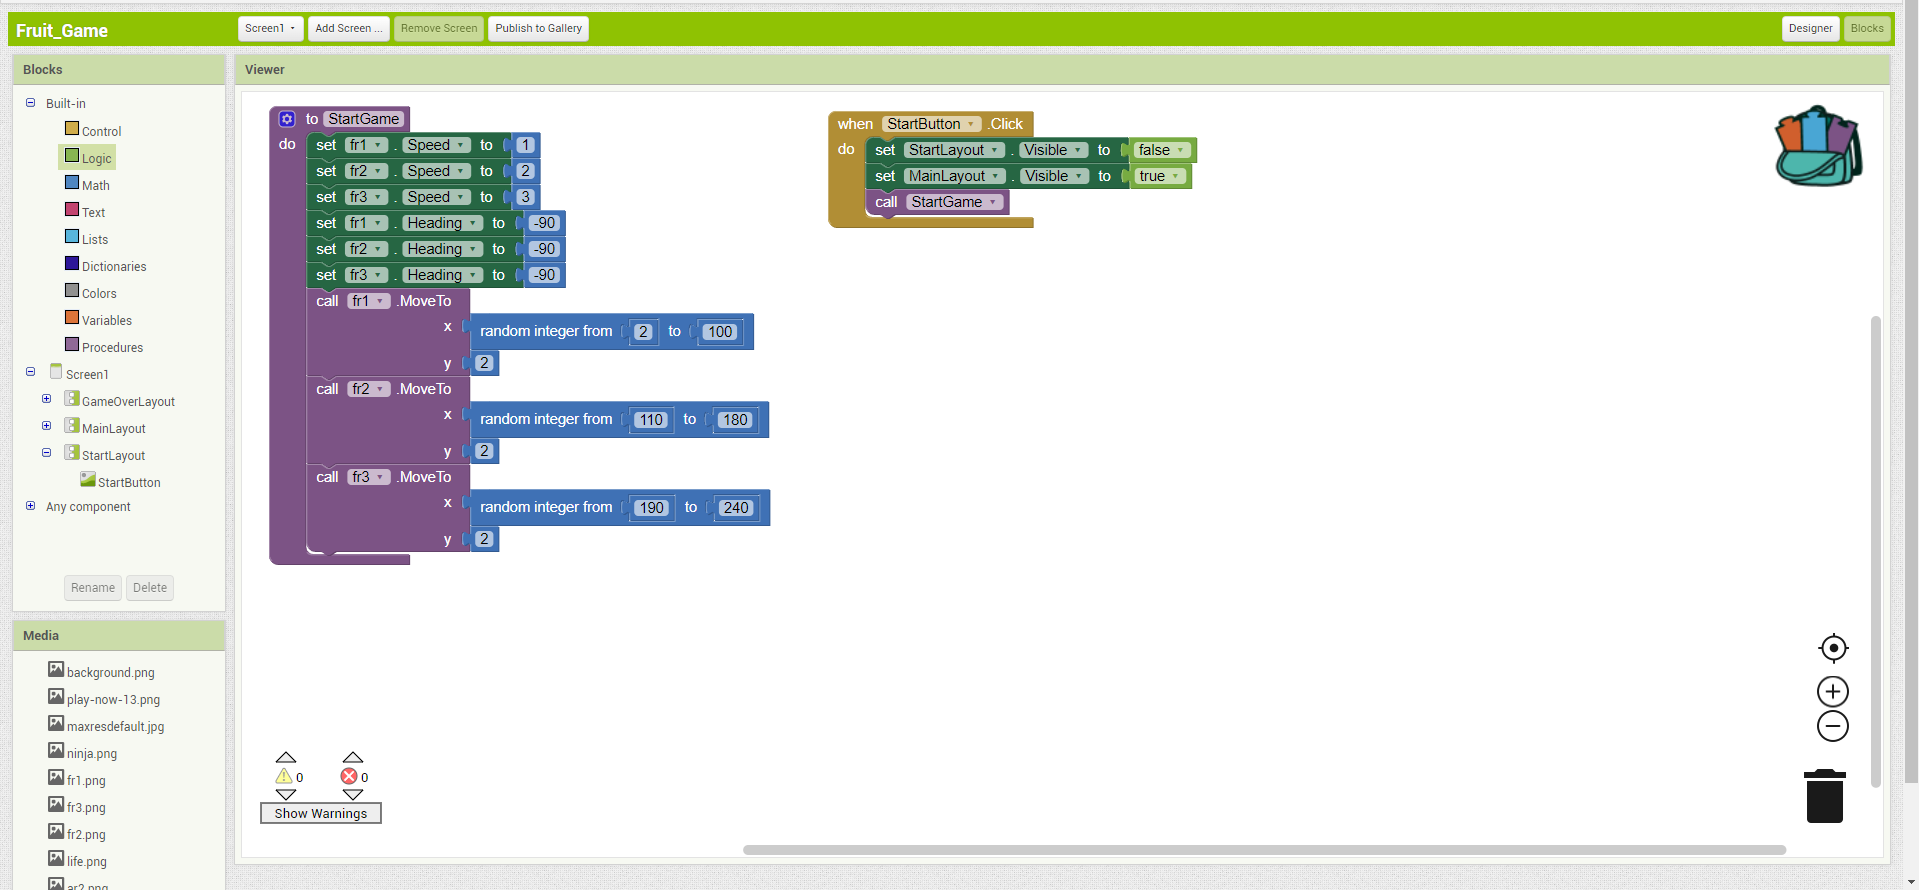
\includegraphics[width=1.0\linewidth,height=0.5\linewidth]{fig120017.png}
   \caption{Programming the start game button}
\label{fig120017}
\end{figure}

The game character will move left and right when clicking the left or right arrows. For this purpose, two events should be added - when a left arrow or right arrow is clicked. The instructions in these two events are similar - the character must change his position relative to the X coordinate. In one case, it should increase; in the other, it should decrease.

\begin{figure}[H]
   \centering
   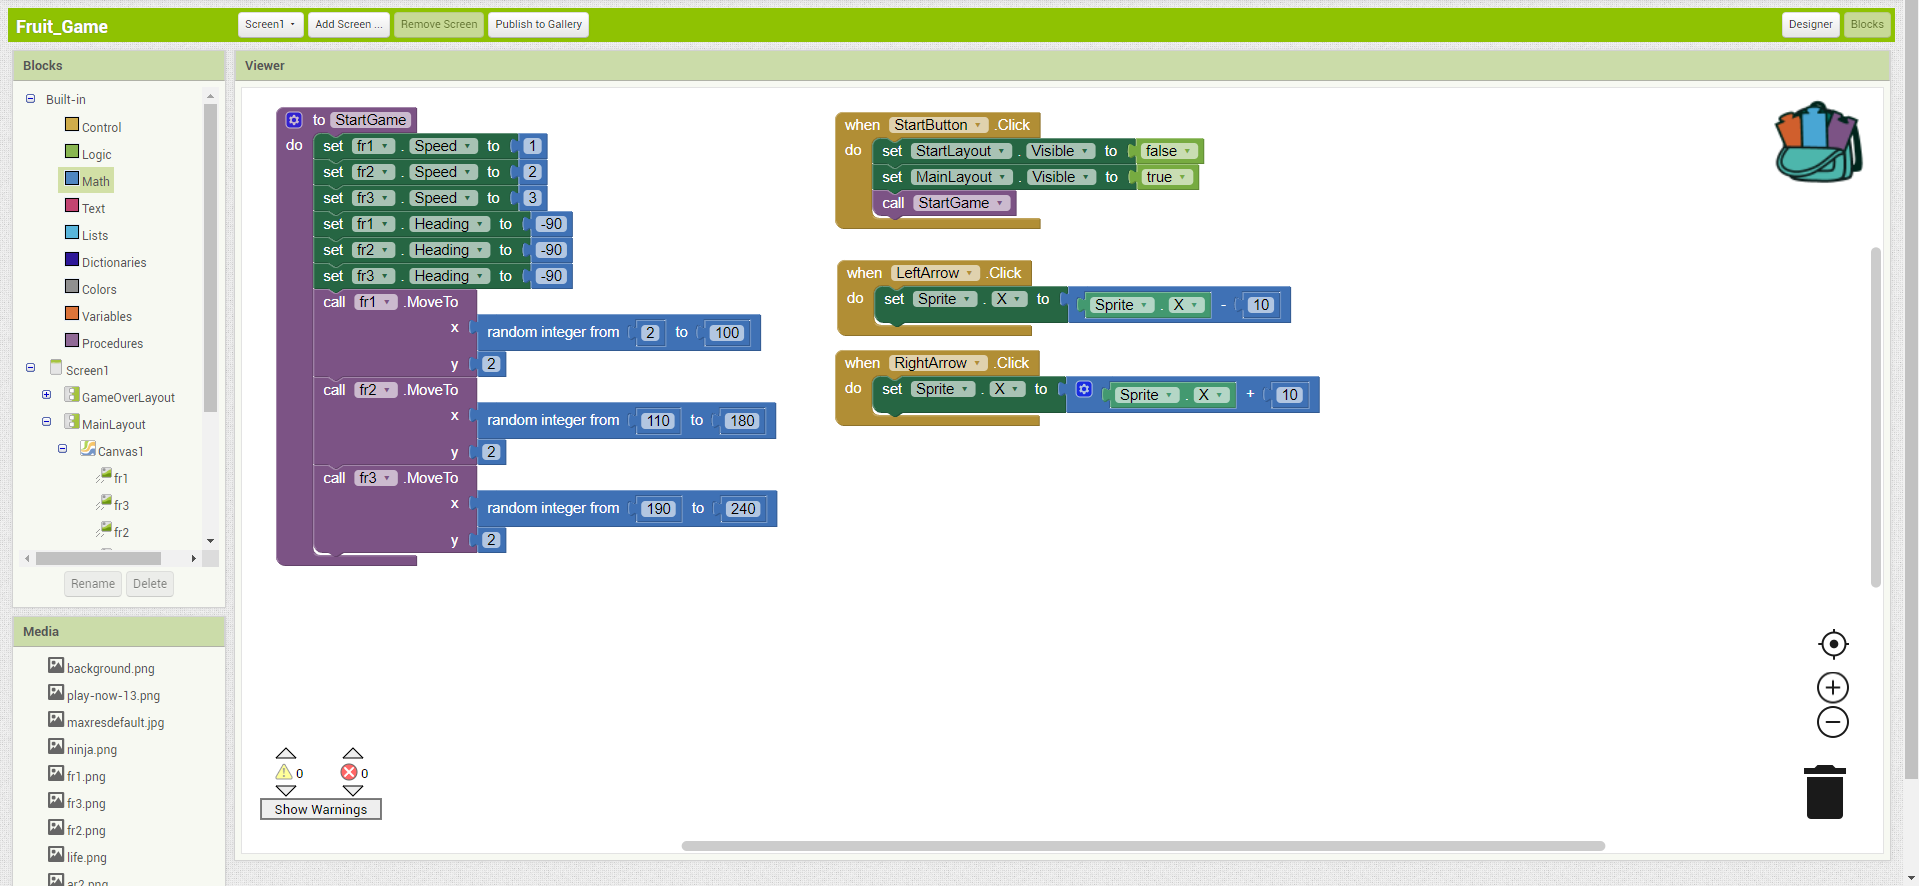
\includegraphics[width=1.0\linewidth,height=0.5\linewidth]{fig120018.png}
   \caption{Programming the character to move}
\label{fig120018}
\end{figure}

In this game, the following variables must be created - 3 that will be responsible for the speed of the three fruits and one for the hero's life.

\begin{figure}[H]
   \centering
   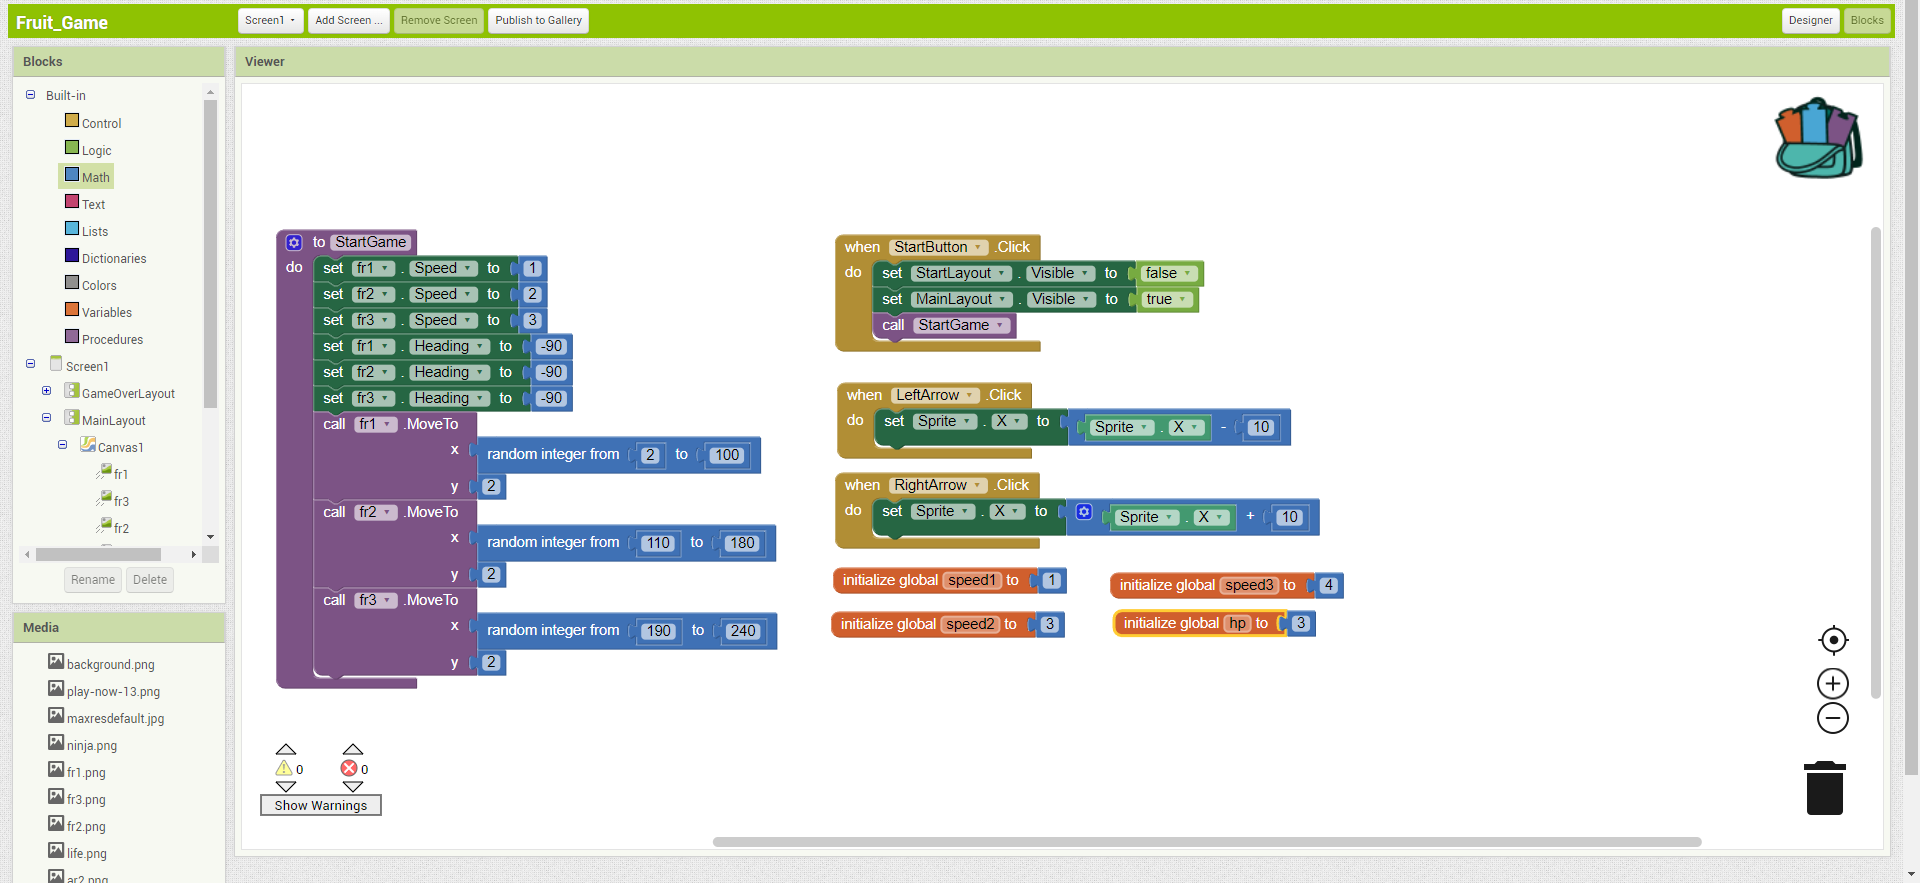
\includegraphics[width=1.0\linewidth,height=0.5\linewidth]{fig120019.png}
   \caption{Adding variables to the game}
\label{fig120019}
\end{figure}

When the player touches a fruit, his points will increase. A procedure will again be constructed since the instruction that changes the points must be called for all three fruits.

\begin{figure}[H]
   \centering
   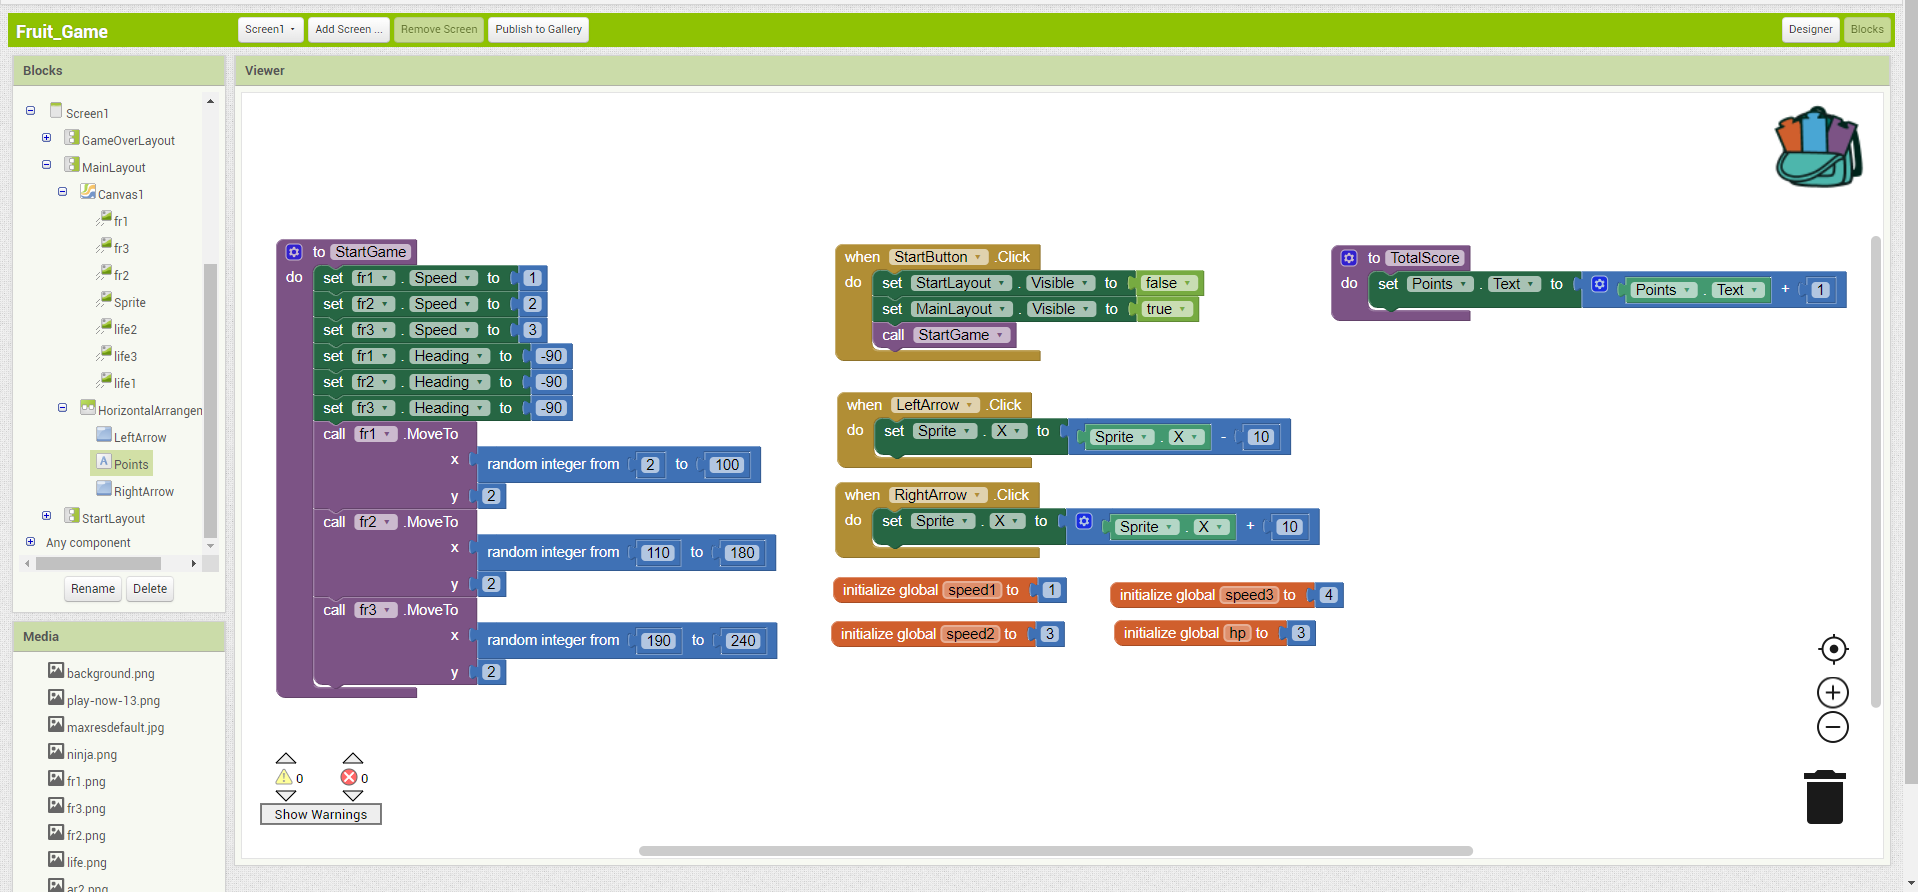
\includegraphics[width=1.0\linewidth,height=0.5\linewidth]{fig120020.png}
   \caption{Procedure for changing points}
\label{fig120020}
\end{figure}

In the next step, instructions will be added to execute when the player touches a fruit. The algorithm is as follows: the fruit's position is changed, the points are increased by 1 (a procedure is created), and the character's speed increases.

\begin{figure}[H]
   \centering
   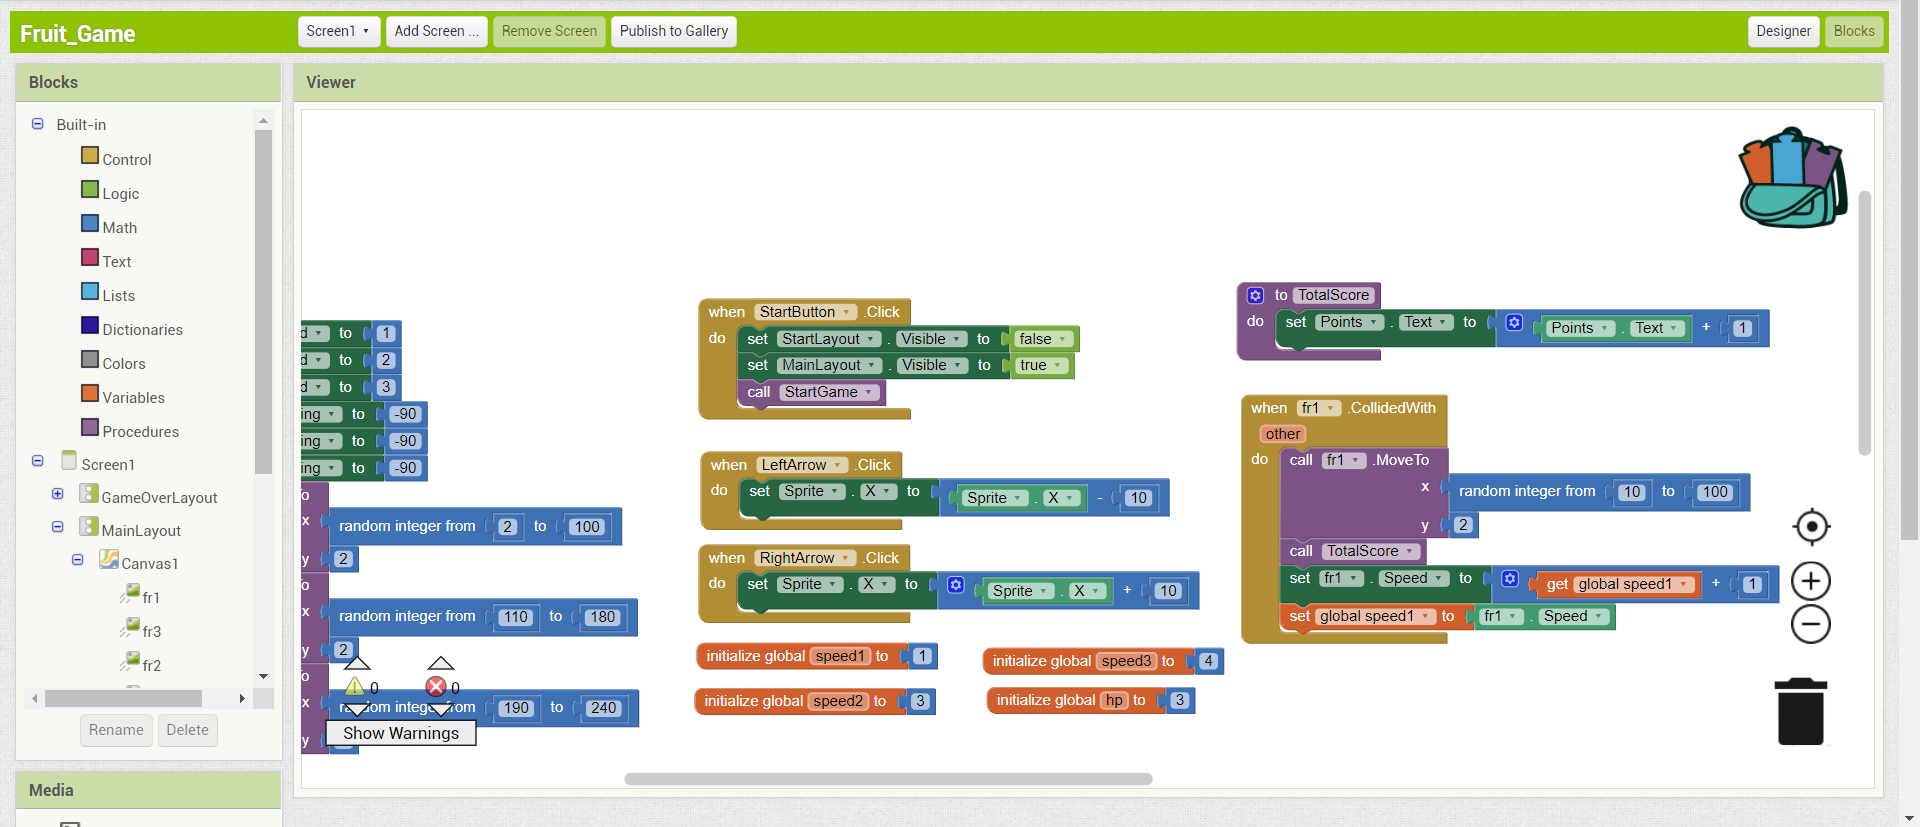
\includegraphics[width=1.0\linewidth,height=0.5\linewidth]{fig120021.png}
   \caption{Algorithm when the player touches fruit}
\label{fig120021}
\end{figure}

This algorithm should also be constructed for the other fruit characters.

\begin{figure}[H]
   \centering
   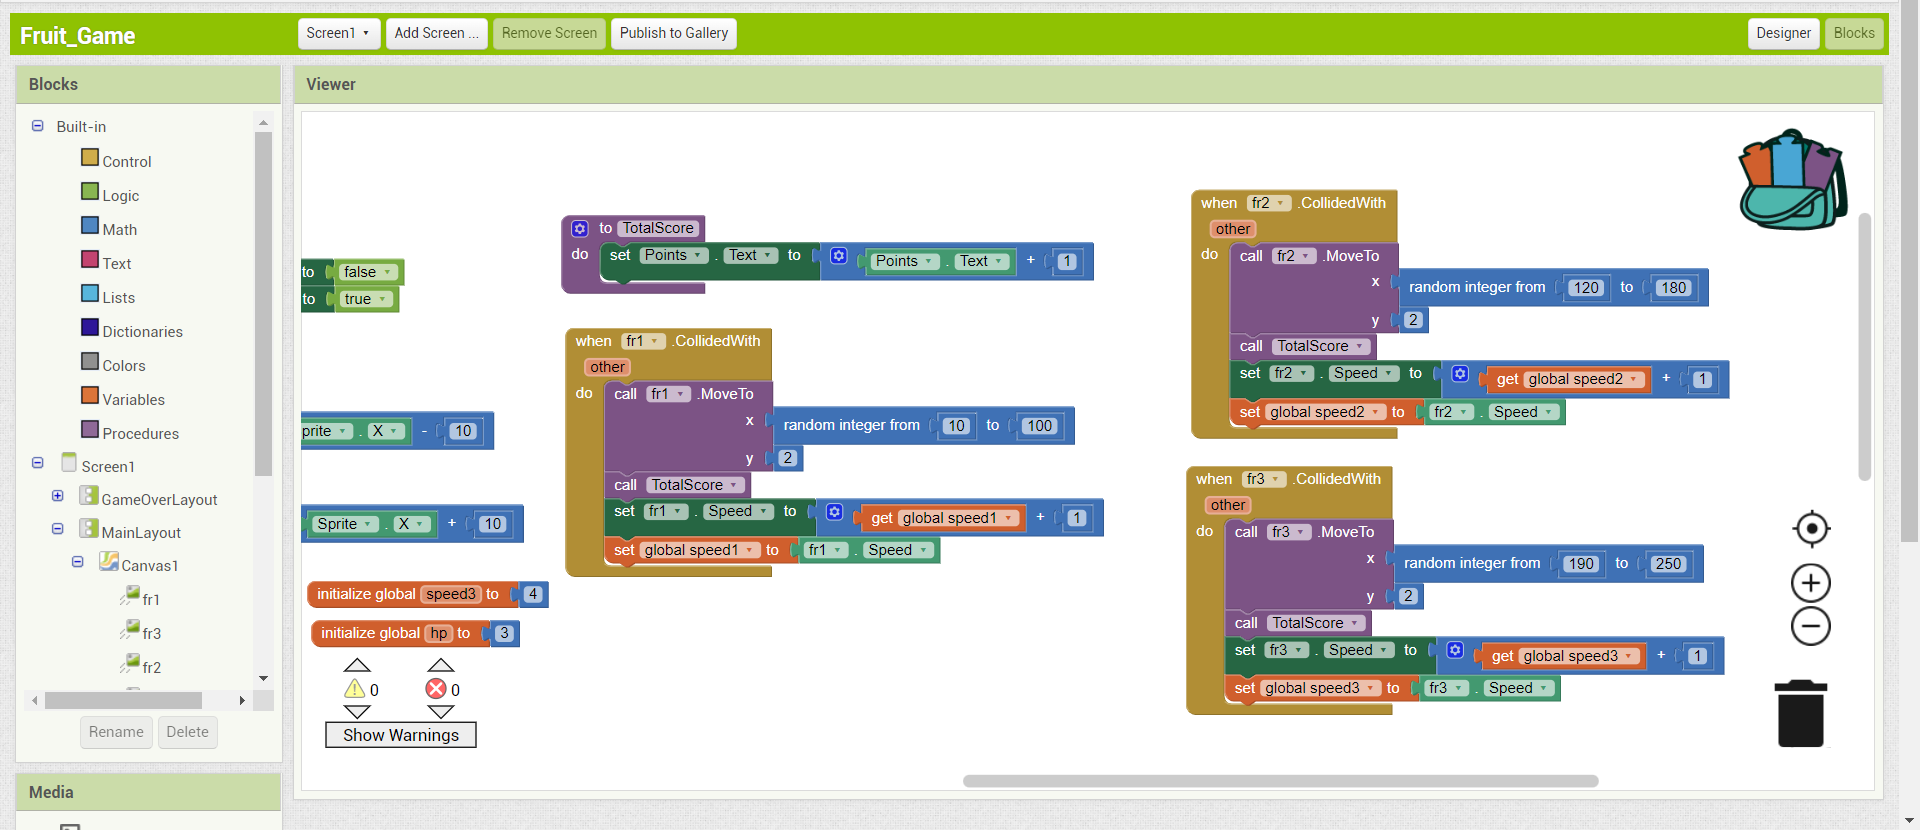
\includegraphics[width=1.0\linewidth,height=0.5\linewidth]{fig120022.png}
   \caption{The All Fruit Algorithm}
\label{fig120022}
\end{figure}

The last procedure to create is to check if the game should end. If the number of lives equals 0, the main screen should be hidden, and the endgame screen should appear. Also, the speed of all fruits should become equal to 0.

\begin{figure}[H]
   \centering
   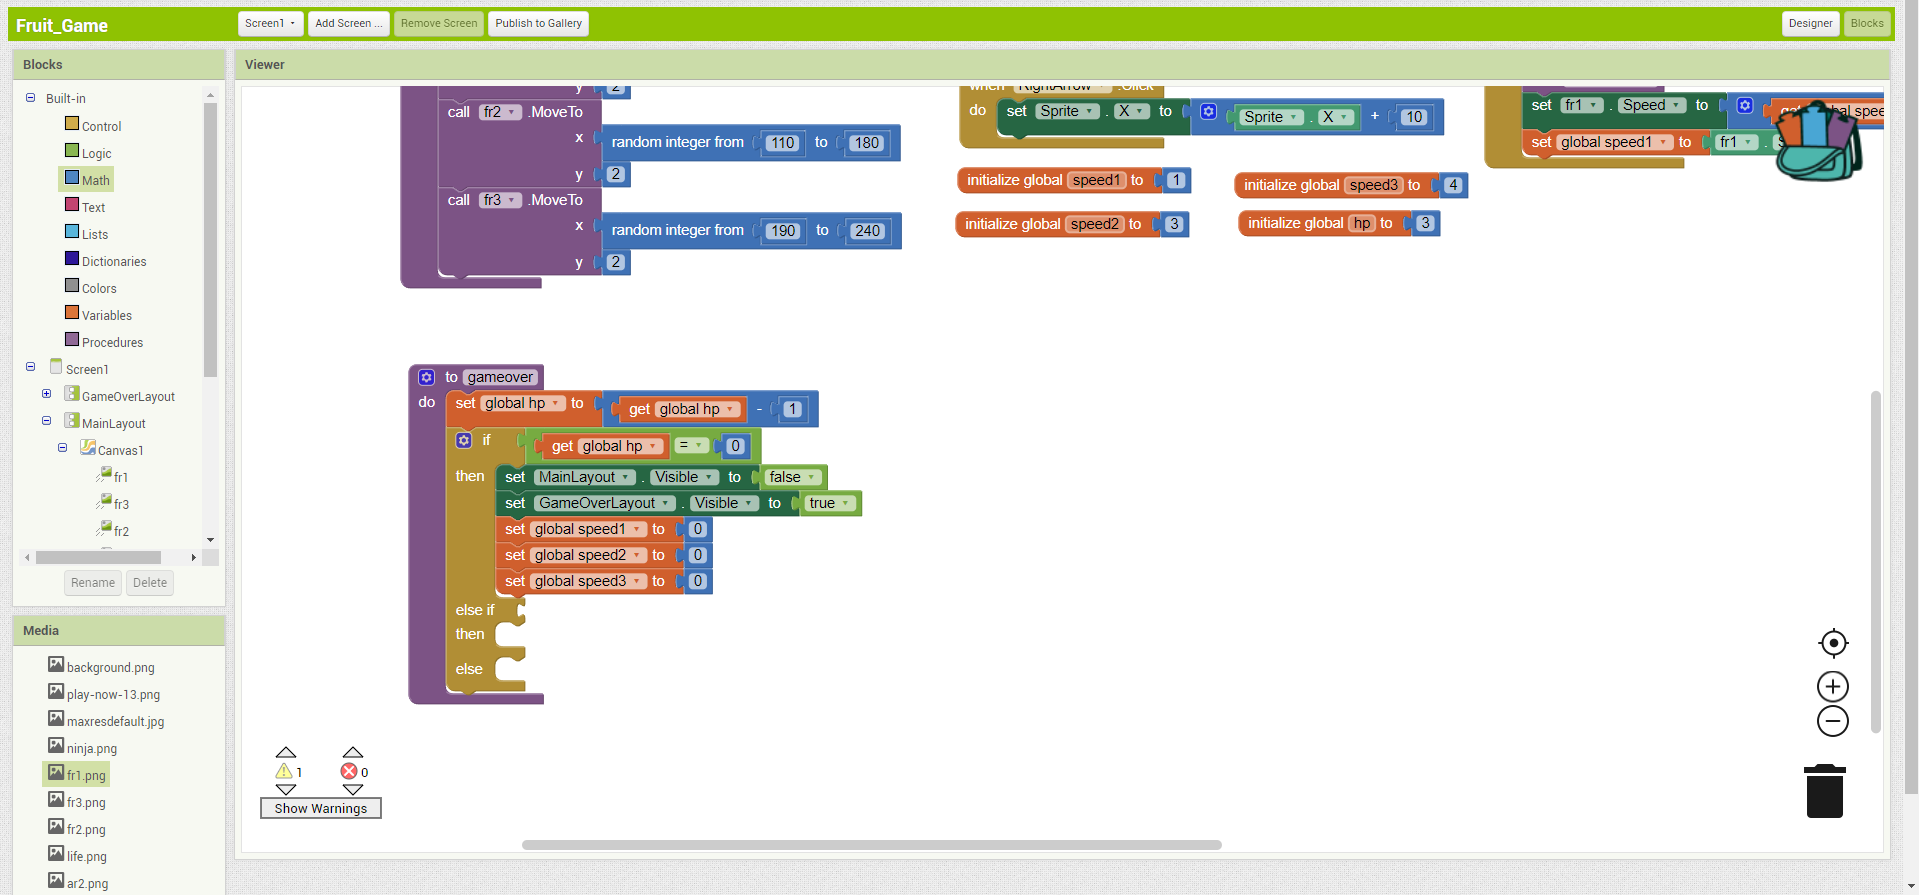
\includegraphics[width=1.0\linewidth,height=0.5\linewidth]{fig120023.png}
   \caption{Checking if the character loses the game}
\label{fig120023}
\end{figure}

Checks should be made if the lives are 2 or 1. If there are two, the player has lost 1 and must hide one of the lives. Again the Visible property needs to be changed. If the number is 1, the player has lost 2 lives, and the picture of one more life should be hidden.

\begin{figure}[H]
   \centering
   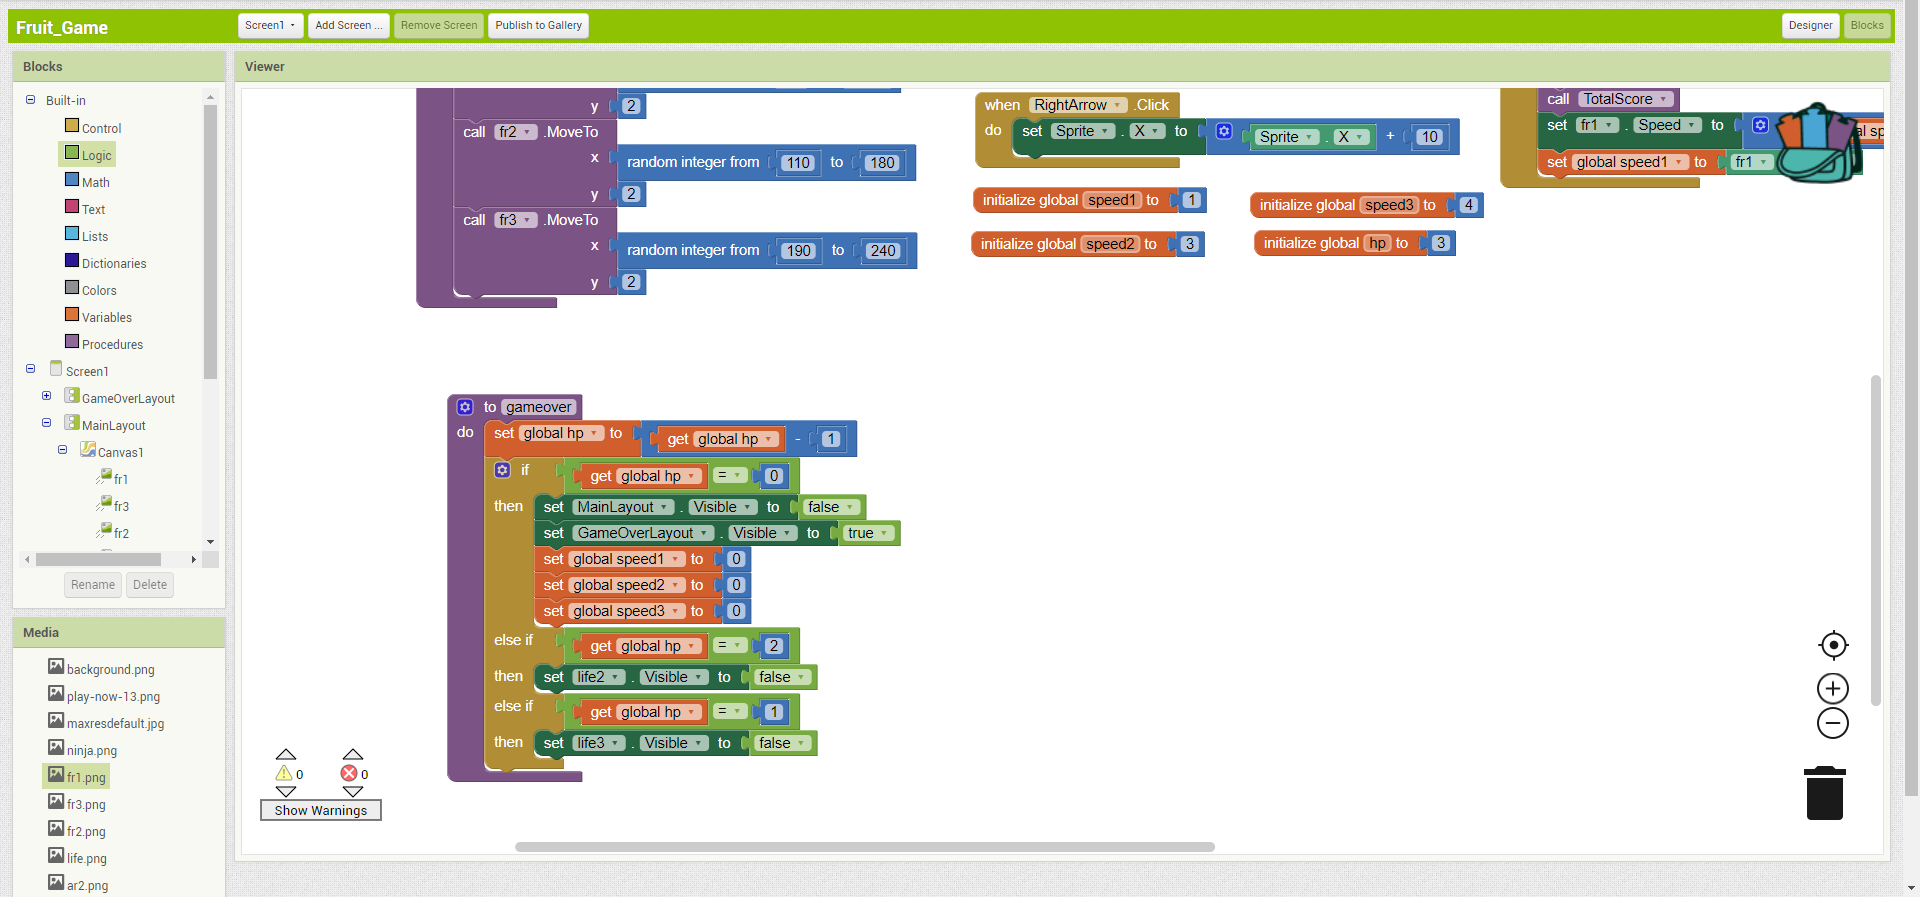
\includegraphics[width=1.0\linewidth,height=0.5\linewidth]{fig120024.png}
   \caption{Checking if the character has life}
\label{fig120024}
\end{figure}

When the fruit character touches the end of the screen, then the endgame check procedure should be called and change its position.

\begin{figure}[H]
   \centering
   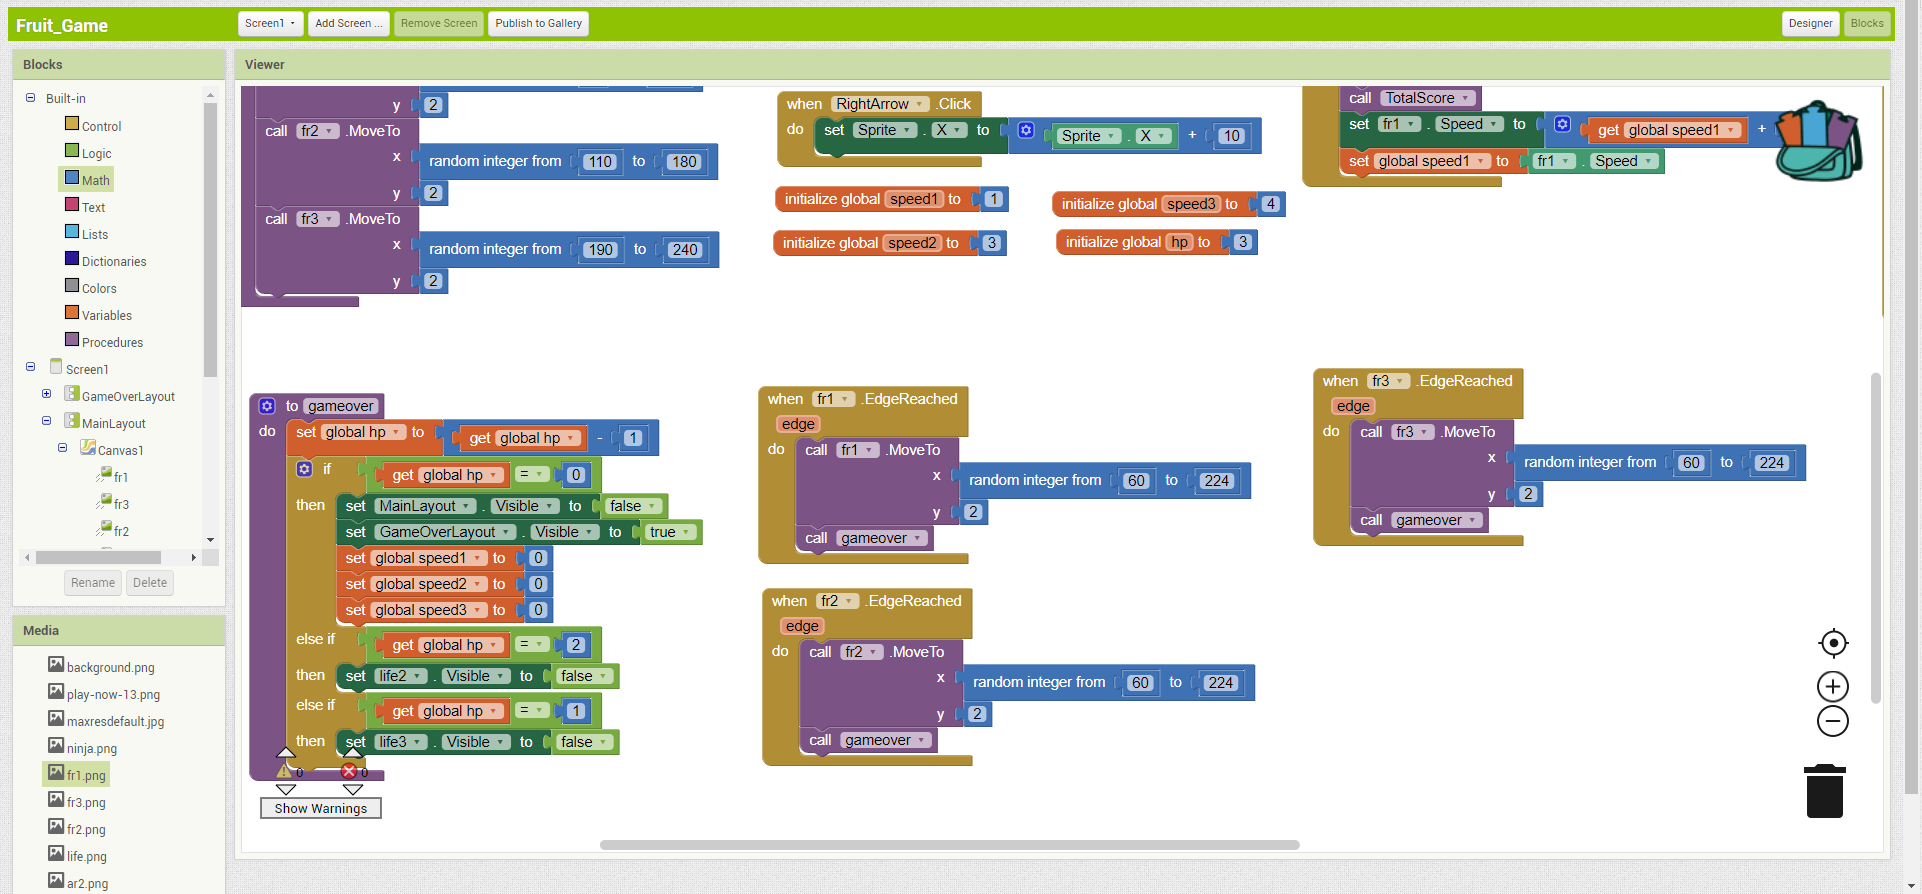
\includegraphics[width=1.0\linewidth,height=0.5\linewidth]{fig120025.png}
   \caption{Checking if a fruit has touched the edge}
\label{fig120025}
\end{figure}

The last instructions to be constructed are when the game is over, and the player presses the restart game button.

\begin{figure}[H]
   \centering
   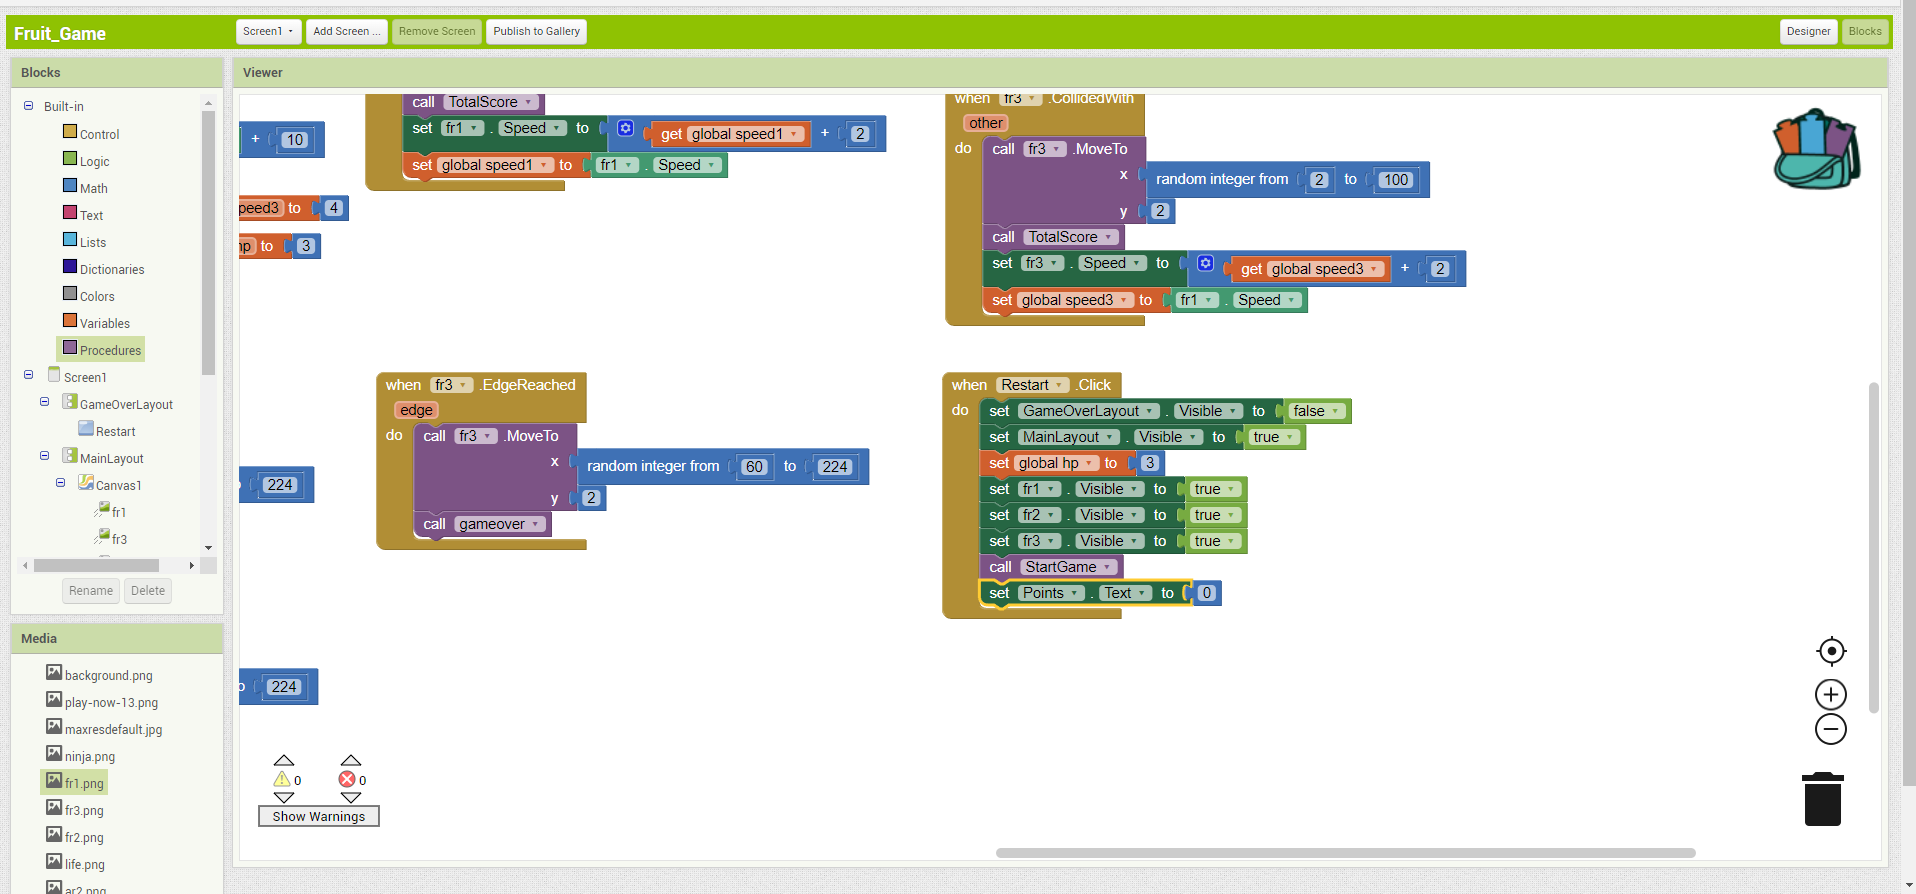
\includegraphics[width=1.0\linewidth,height=0.5\linewidth]{fig120026.png}
   \caption{Game Over}
\label{fig120026}
\end{figure}

Game over. It should be tested on the phone.
